\chapter{El LHC y el detector ATLAS}
% \addcontentsline{toc}{chapter}{El LHC y el detector ATLAS}
\chaptermark{El LHC y el detector ATLAS}



El Gran Colisionador de Hadrones (\textit{\textbf{L}arge \textbf{H}adron \textbf{C}olider} (LHC)) \cite{Evans:1129806} es el acelerador de hadrones de la Organización Europea para la Investigación Nuclear (CERN, por sus antiguas siglas en francés), ubicado en la frontera entre Francia y Suiza. Posee una longitud de 27 km y fue construido en el mismo túnel en el que funcionaba el acelerador $e^{+}e^{-}$ LEP (entre 1989 y 2000) \cite{LEPbook}, a una profundidad variable entre $50$ y $174$ m de la superficie.

El LHC está diseñado para colisionar protones (e iones pesados) a una energía de centro de masa de $\sqrt{s}=14 \etev$. Para ello el CERN posee un complejo de aceleradores que, en sucesivas etapas, incrementan la energía de los protones (Figura \ref{acc_complex}). El último de los aceleradores es el LHC, donde los protones circulan en direcciones opuestas por cavidades de ultra alto vacío a una presión de $10^{-10}$ torr. El mismo cuenta con $1232$ dipolos magnéticos superconductores enfriados a $1.9$ K, que generan un campo magnético de $8.4$ T, lo que permite mantener en su órbita circular a los protones. Los dipolos están equipados con sextupolos, octupolos y decapolos, que permiten corregir las pequeñas imperfecciones del campo magnético en las extremidades de los dipolos. Para aumentar la probabilidad de colisión, existe un sistema de focalización de los haces en las proximidades de los detectores, que estrecha el camino que recorren los protones. El mismo consiste de $392$ cuadrupolos magnéticos que generan campos magnéticos de $6.8$ T. 

\begin{figure}
\centering
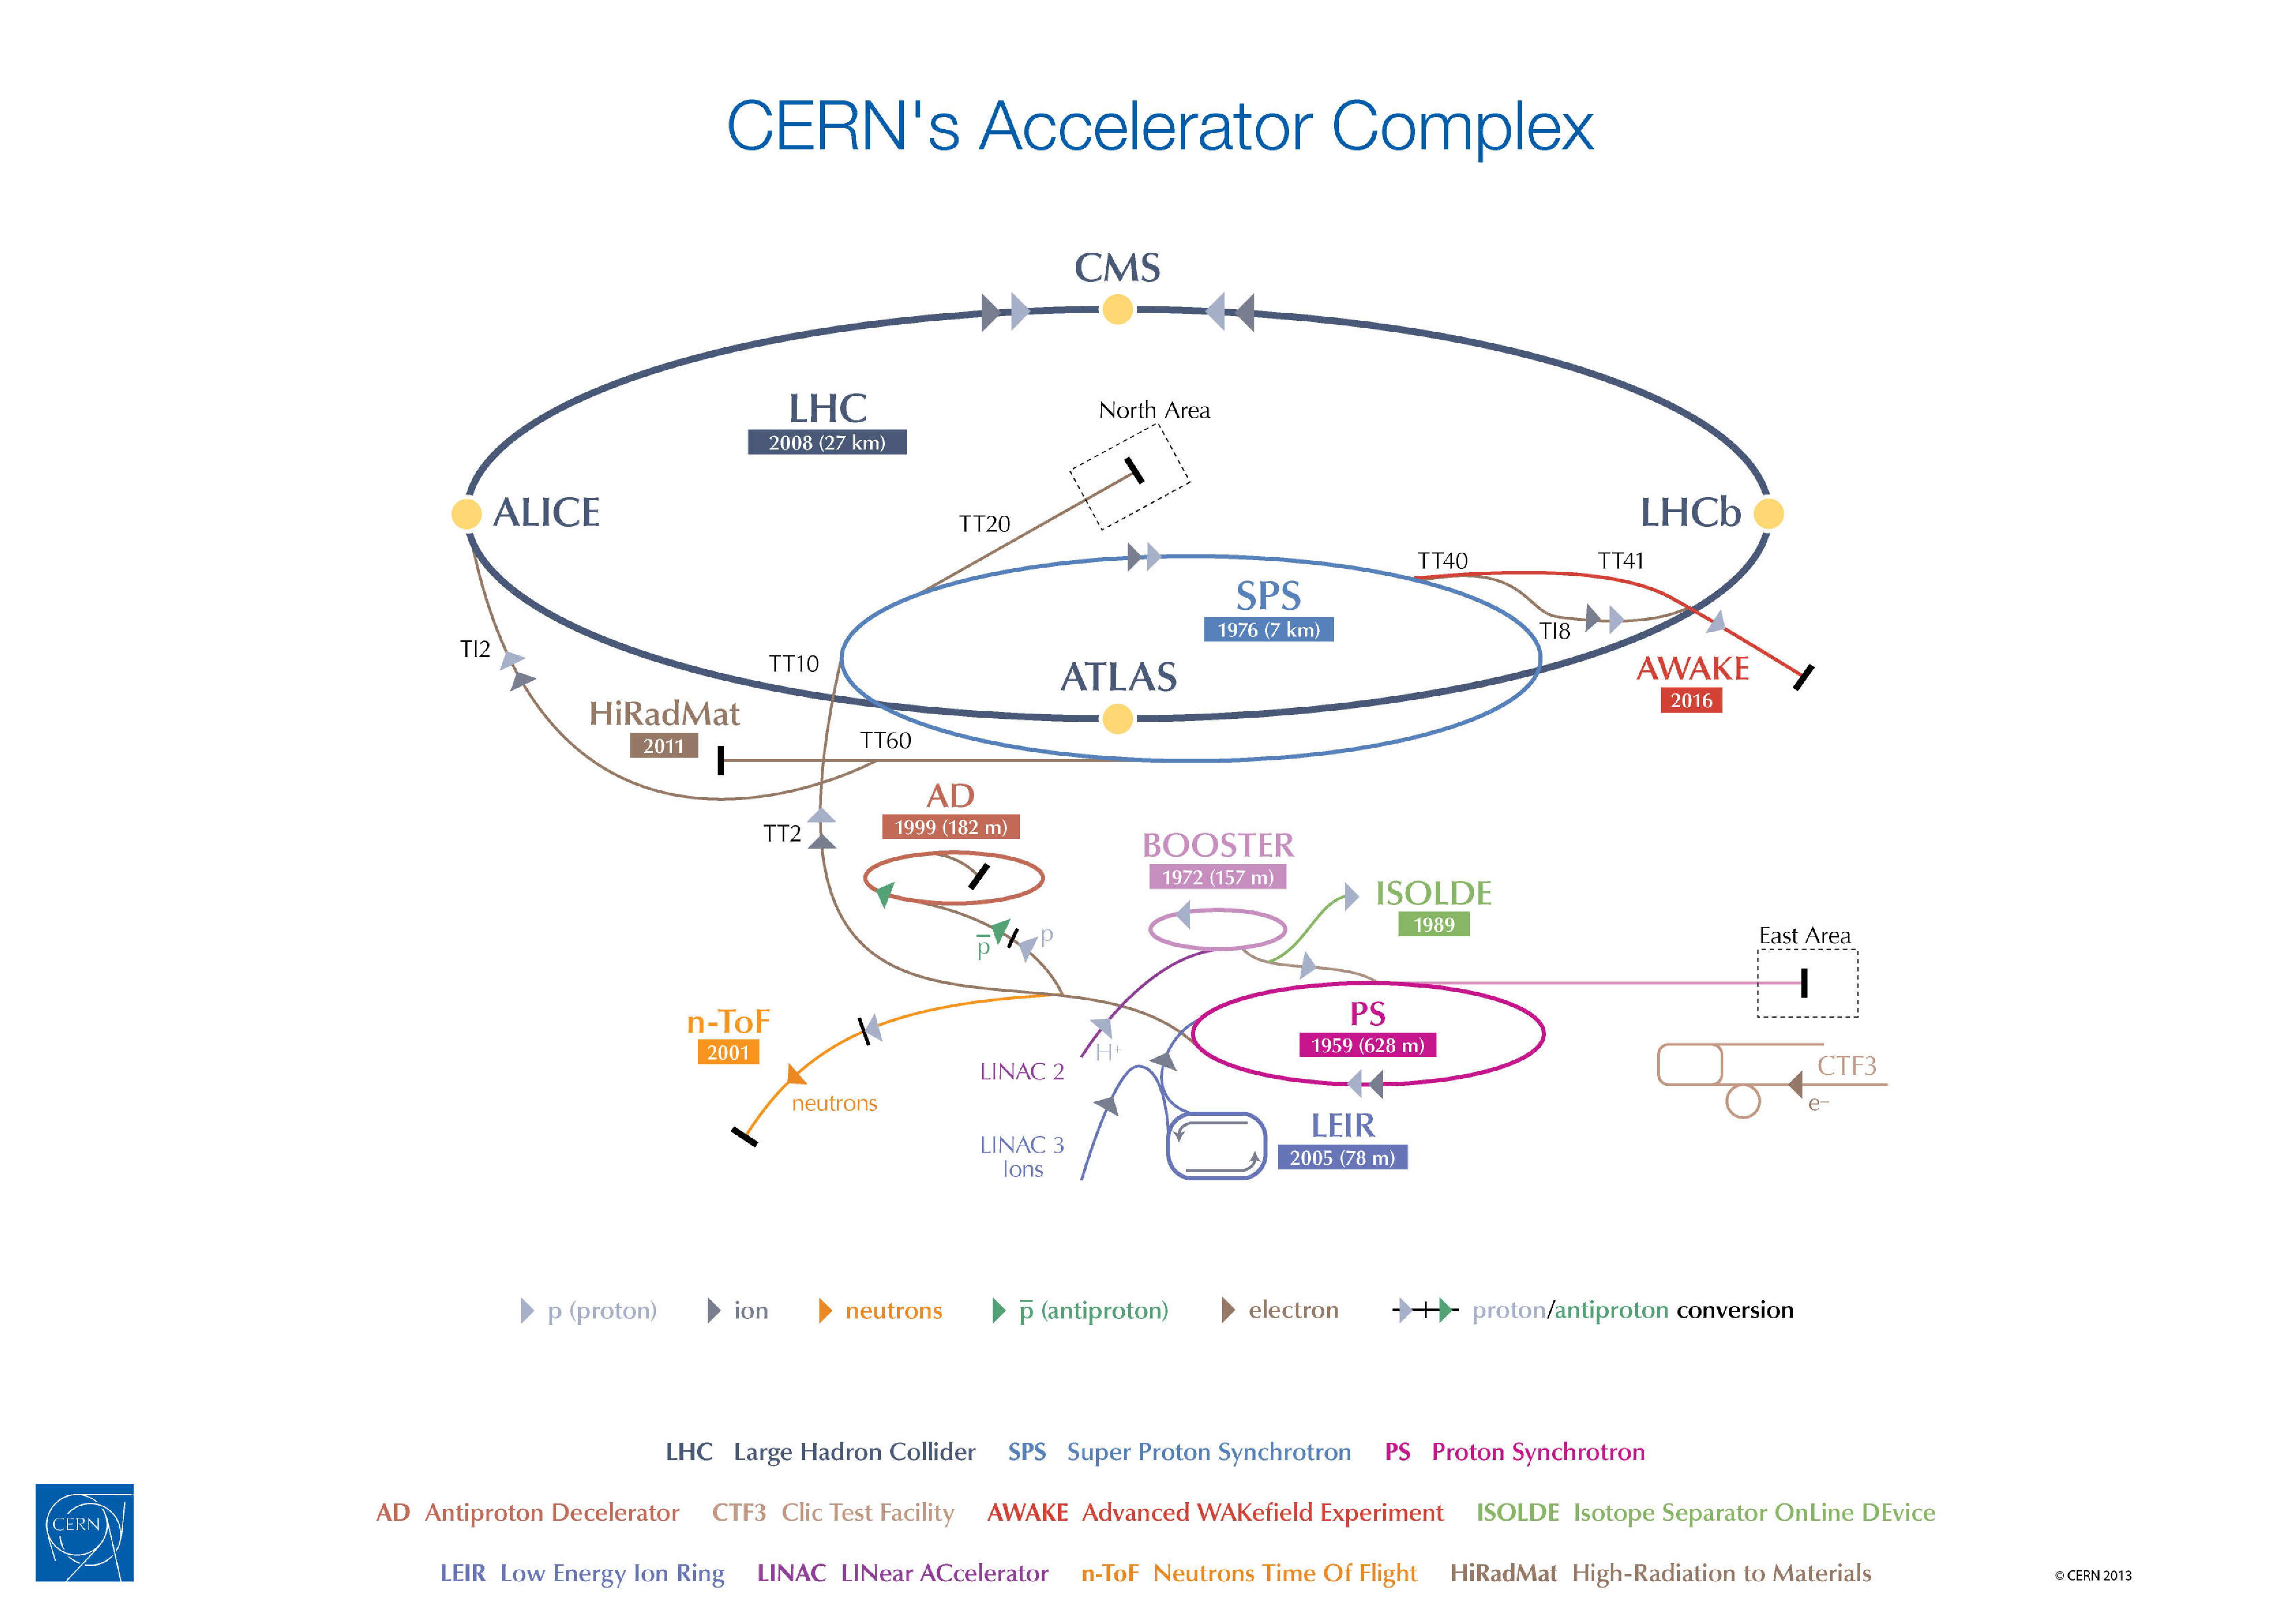
\includegraphics[width=1\textwidth]{acc_complex-eps-converted-to.pdf}
\caption{Complejo de aceleradores del CERN, incluyendo al LHC y a la serie de aceleradores utilizados para proveer de protones al LHC. También pueden verse los diferentes experimentos ubicados en distintos puntos del acelerador.}
\label{acc_complex}
\end{figure}

El diseño del LHC contempla trenes de $2808$ paquetes de $\sim 10^{11}$ protones cada uno, espaciados temporalmente en $25$ ns. Para caracterizar el funcionamiento del acelerador, se utiliza una variable denominada luminosidad instantánea. Se define como el número de partículas por unidad de tiempo y unidad de área:

\begin{equation}
\mathcal{L}=f_{rev}n_{b}\frac{N_{1}N_{2}}{A}
\end{equation}
% comentario intencional para eliminar sangría
donde $f_{rev}$ es la frecuencia de revolución ($\sim$11 kHz), $n_{b}$ es el número de \textit{bunches} (paquetes de protones) por haz, $N_{i}$ es el número de partículas en cada \textit{bunch} y \textit{A} es la sección efectiva del haz, que puede expresarse en término de los parámetros del acelerador como:

\begin{equation}
A=\frac{4 \pi \epsilon_{n}\beta^{*}}{\gamma F}
\end{equation}
% comentario intencional para eliminar sangría
donde $\epsilon_{n}$ es la emitancia transversal normalizada (la dispersión transversal media de las partículas del  haz en el espacio de coordenadas e impulsos), $\beta^{*}$ es la función de amplitud en el punto de interacción, relacionada al poder de focalización de los cuadrupolos), $\gamma$ es el factor relativista de Lorentz y \textit{F} es un factor de reducción geométrico, debido al ángulo de cruce de los haces en el punto de interacción.


El LHC funciona desde 2009, pero entre 2013 y 2014 no estuvo operativo debido a que se le hicieron remodelaciones para mejorar su desempeño. En el 2015 volvió a funcionar (Run 2), alcanzando una energía por haz de $6.6 \etev$ ($13 \etev$) y una luminosidad de $1.4\cdot 10^{34}$ cm$^{-2}$s$^{-1}$.

\section{El detector ATLAS}

ATLAS (\textit{\textbf{A} \textbf{T}oroidal \textbf{L}HC \textbf{A}paratu\textbf{S}})  \cite{PERF-2007-01} es uno de los experimentos multipropósito del LHC, diseñado para estudiar las colisiones protón-protón a altas energías provistas por el LHC.

El esquema del detector se puede observar en la Figura \ref{ATLAS}. Tiene una simetría aproximadamente cilíndrica, y está compuesto de distintos subdetectores, que cumplen diversas funciones en la identificación de las partículas producidas durante las colisiones (ver Figura \ref{cross_section_2}). En la zona más próxima al haz se encuentra detector interno de trazas (ID), compuesto del Insertable B-Layer (IBL), un detector de píxeles, un detector de bandas de silicio (SCT) y un detector de radiación de transición (TRT). Envolviendo el ID se encuentra un solenoide superconductor que genera un campo magnético de $2$ T, el cual curva la trayectoria de las partículas cargadas para así medir su impulso.

\begin{figure}
\centering
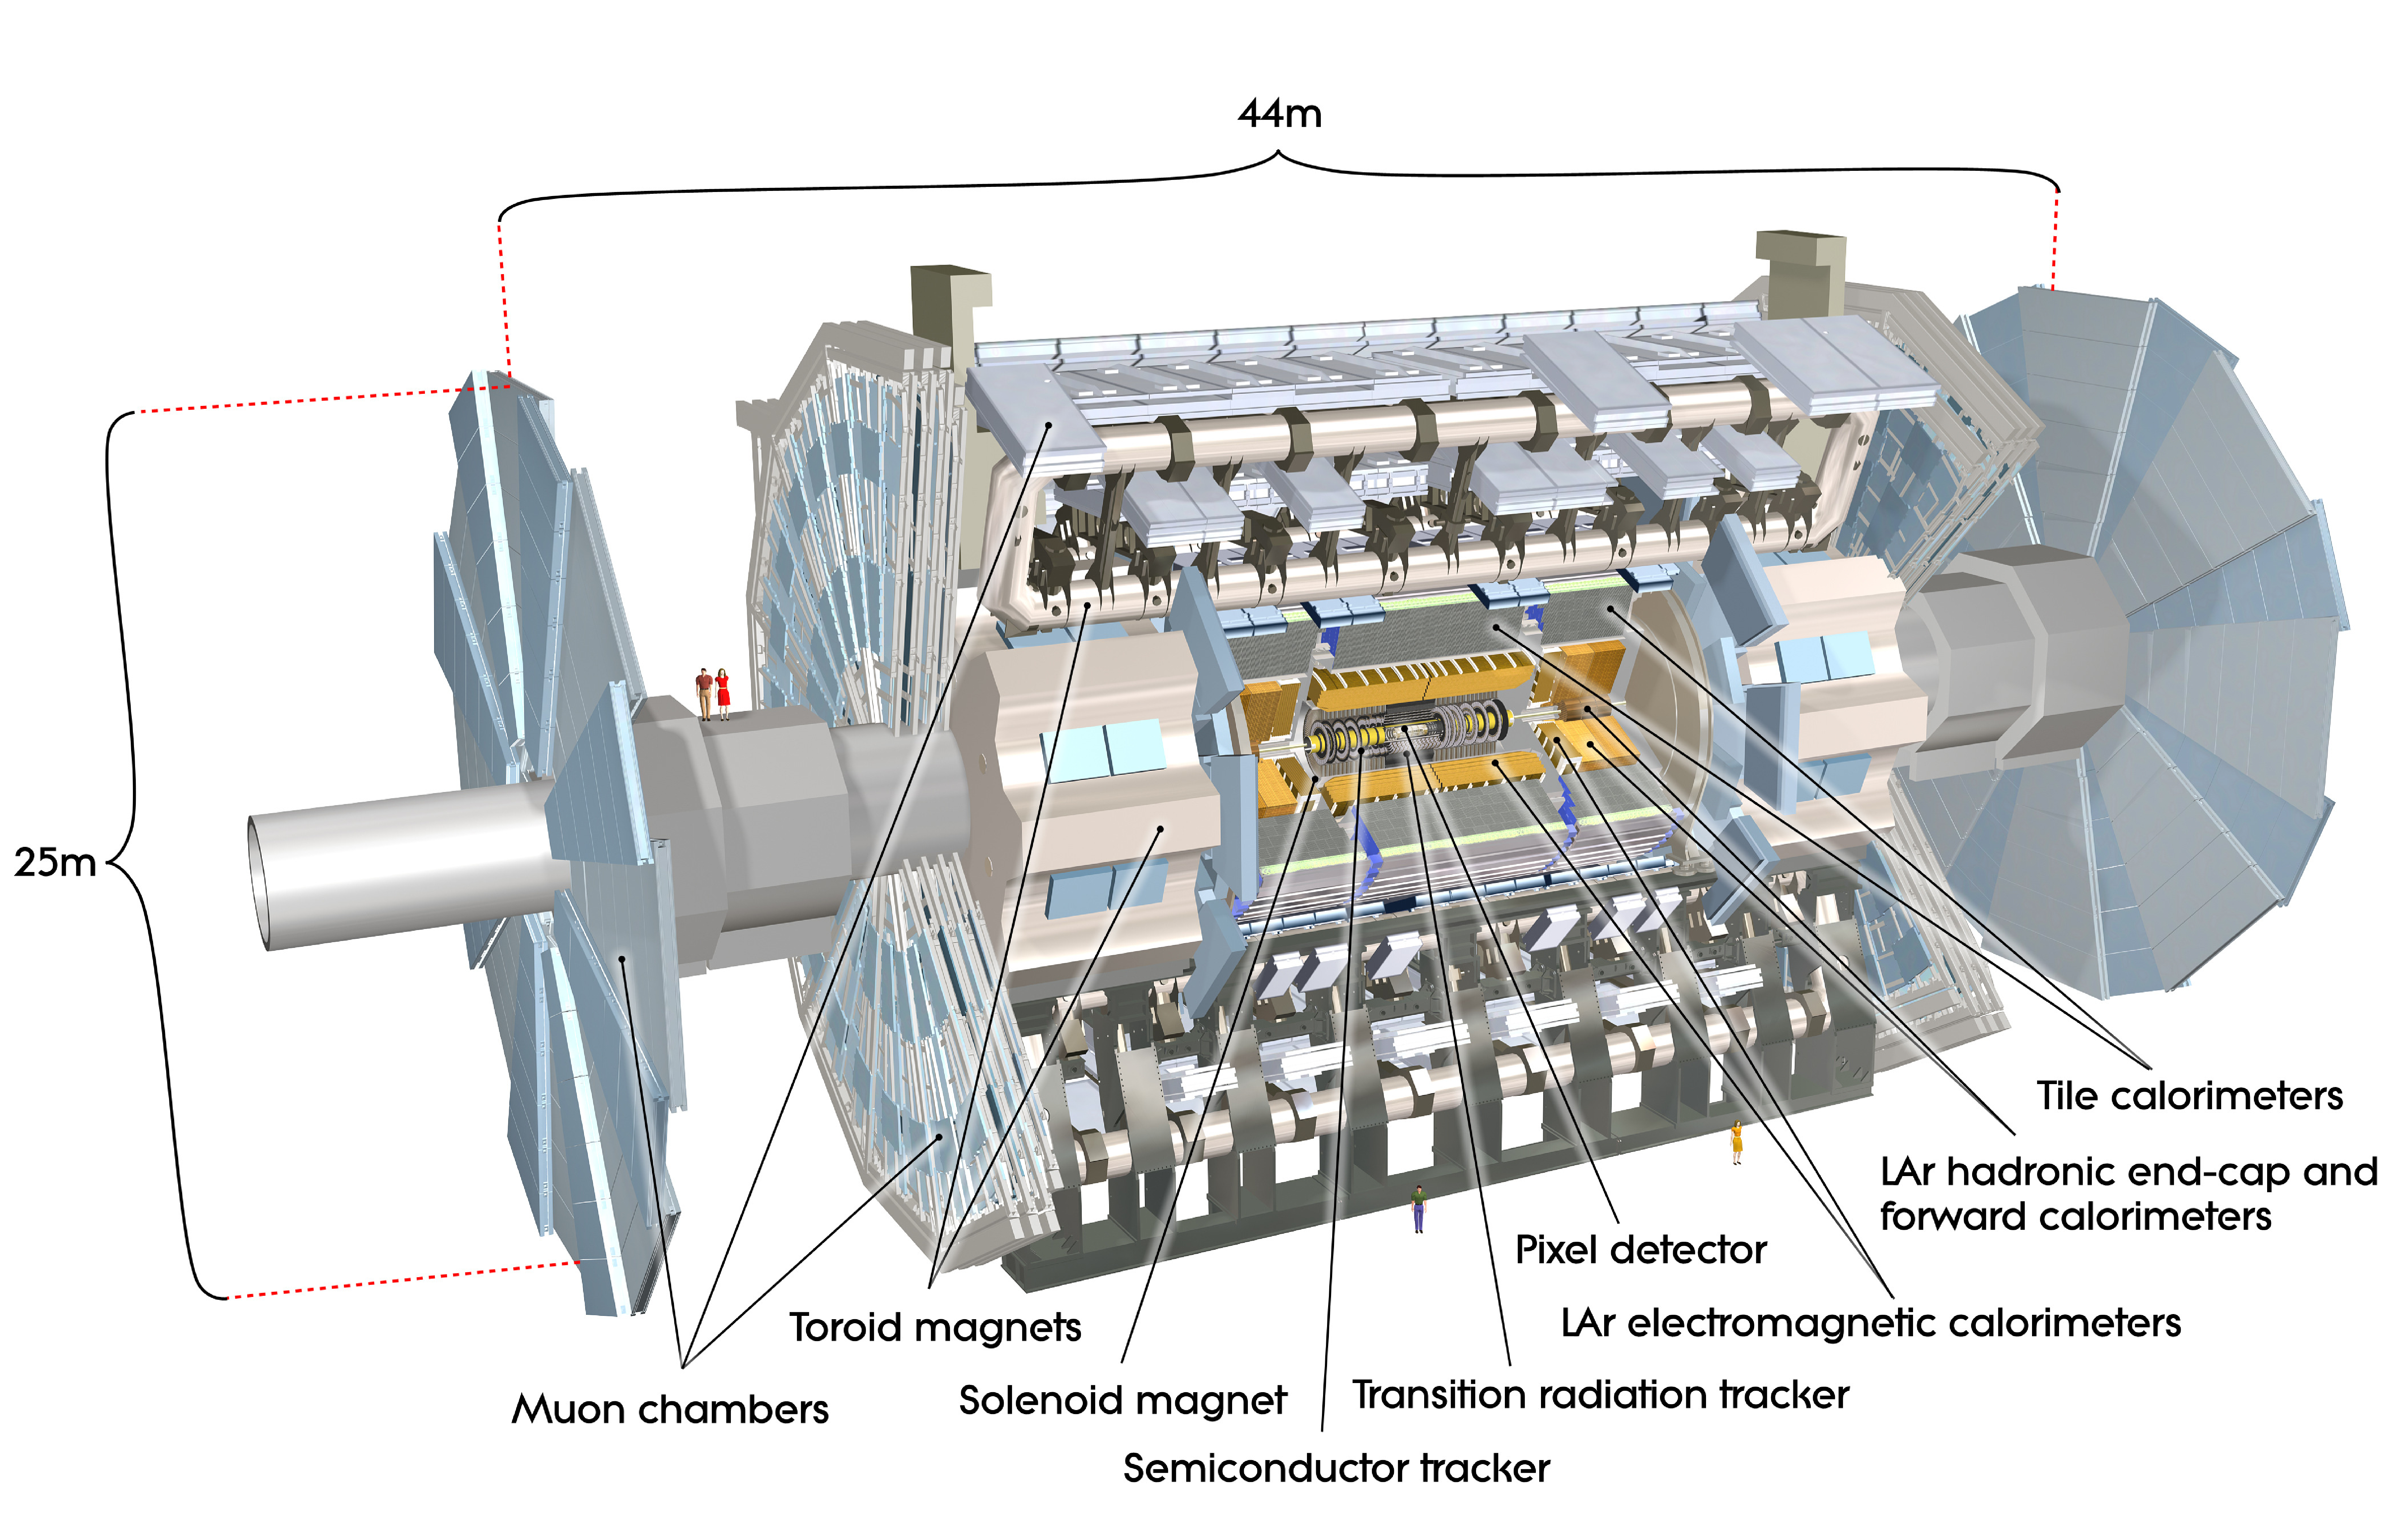
\includegraphics[width=1\textwidth]{ATLAS-eps-converted-to.pdf}
\caption{Esquema general del detector de ATLAS.}
\label{ATLAS}
\end{figure}

\begin{figure}
\centering
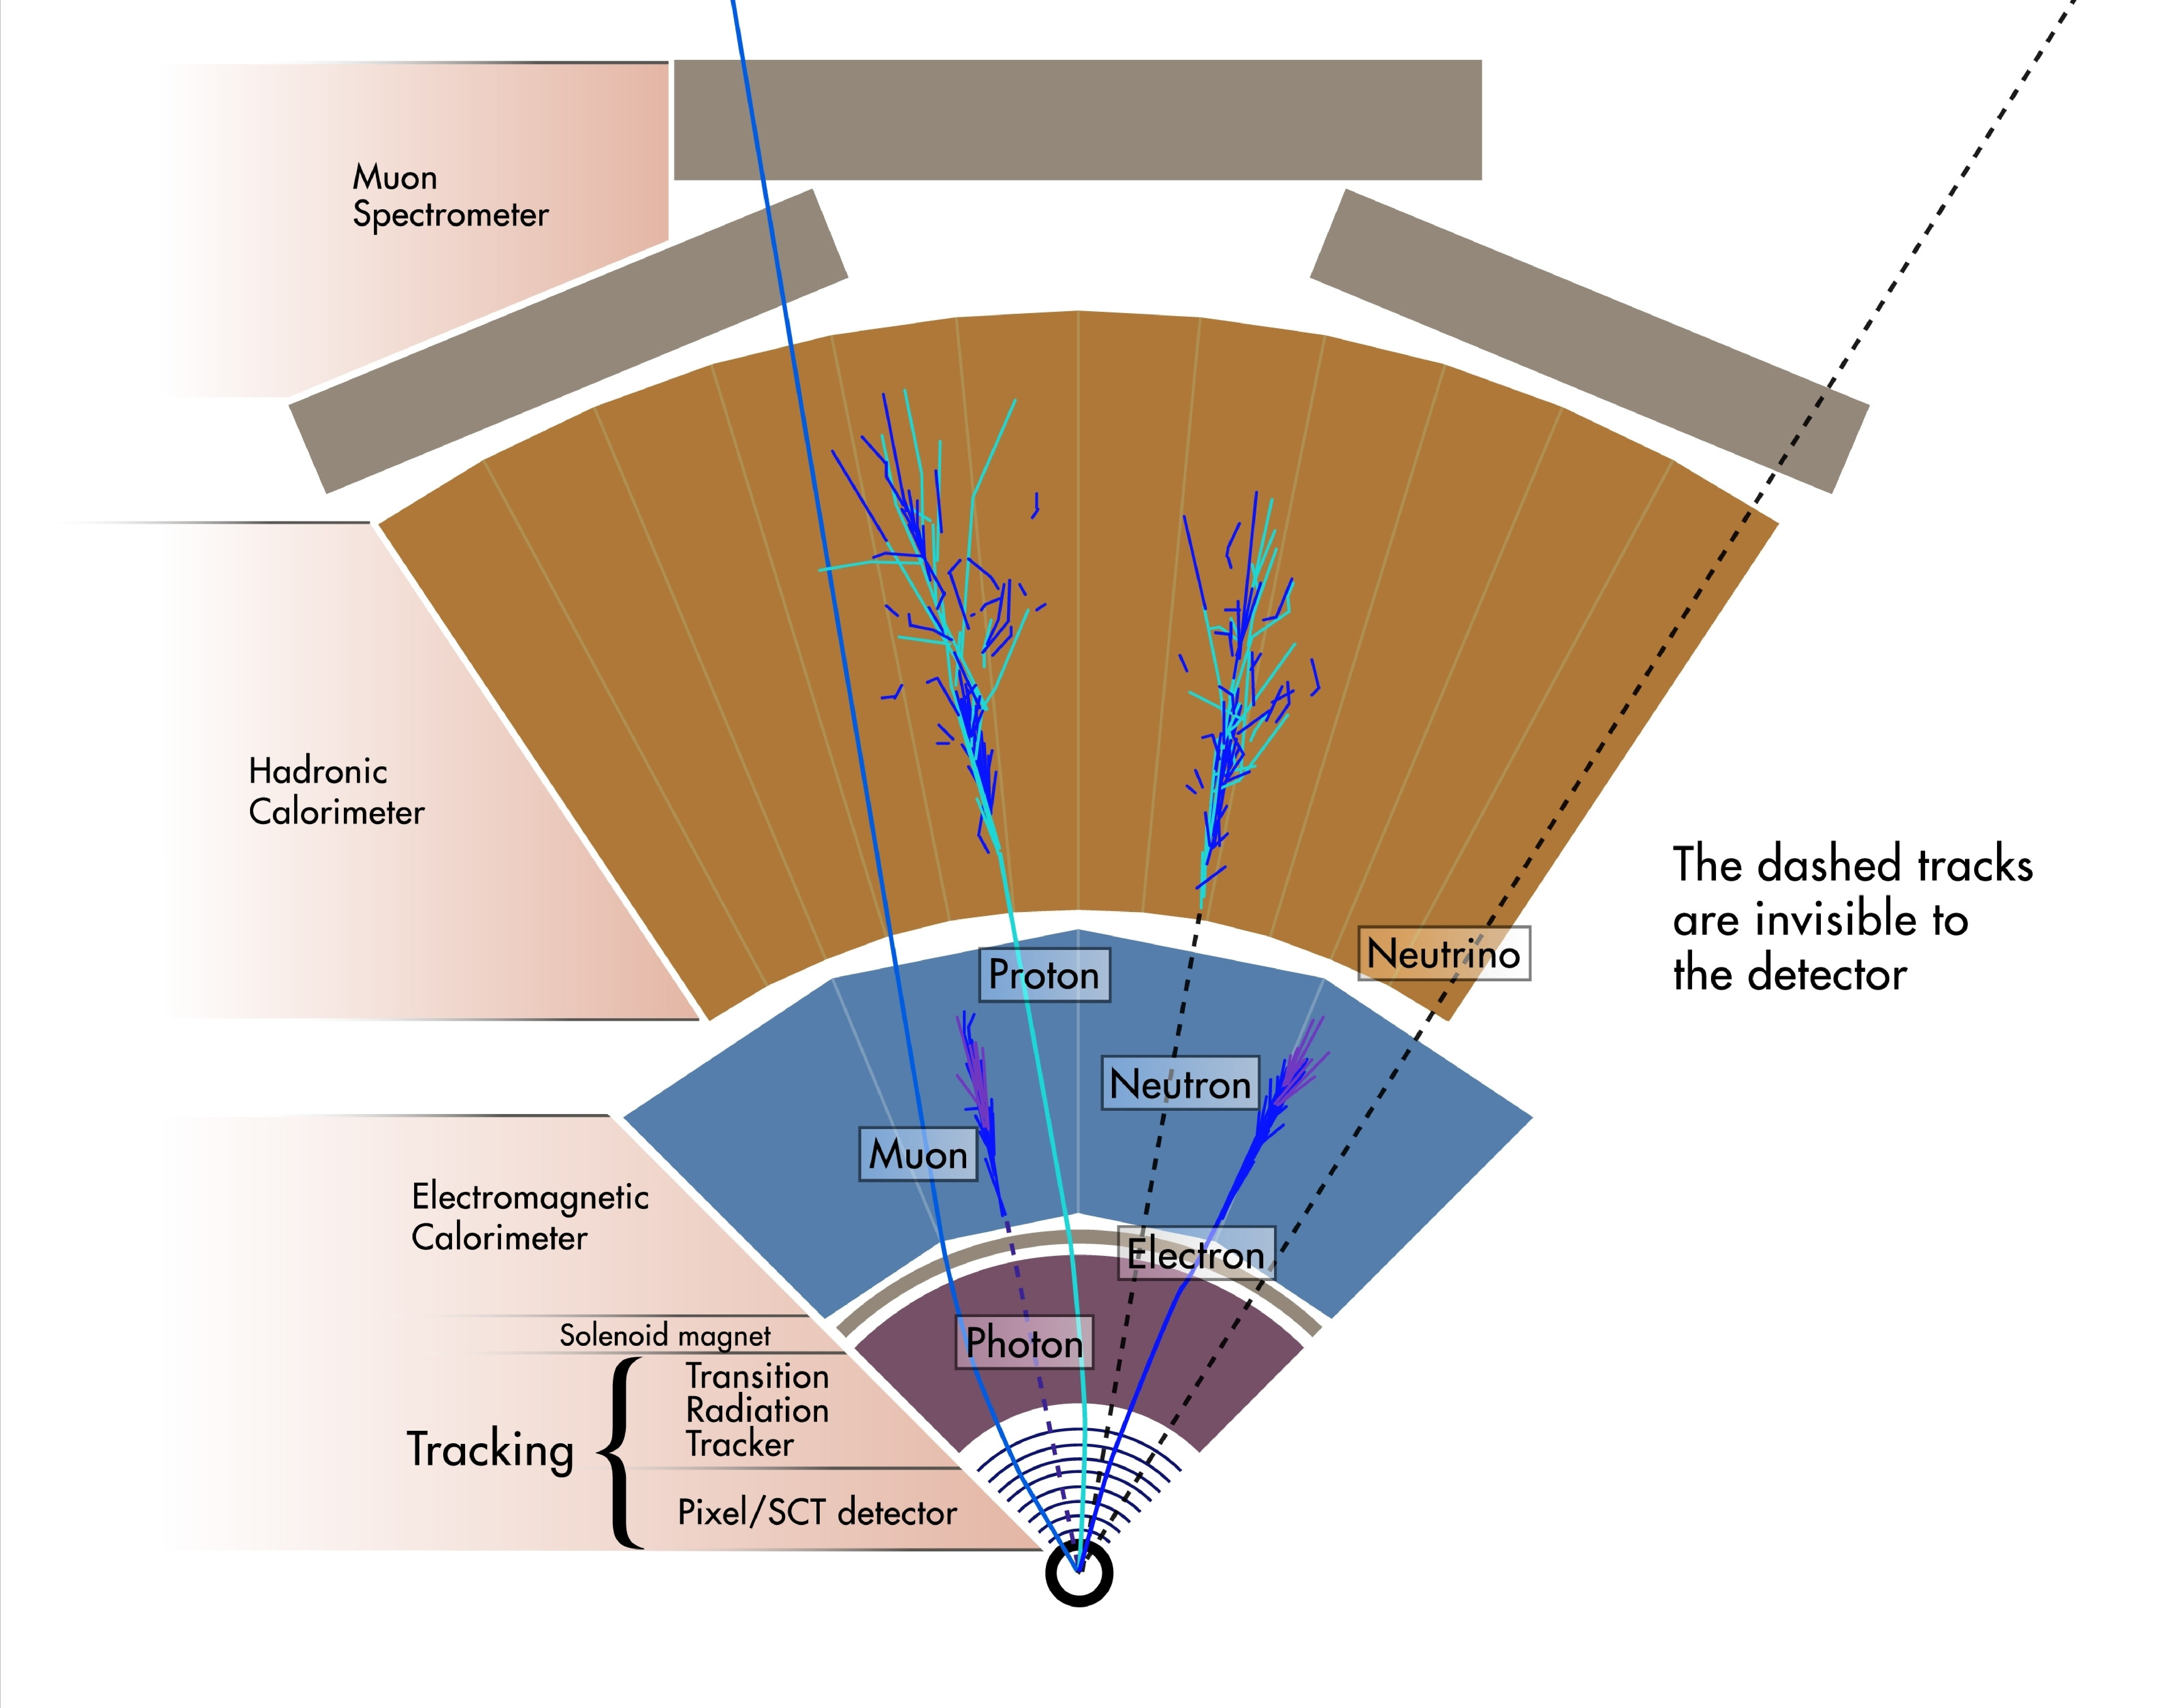
\includegraphics[width=0.7\textwidth]{cross_section_2-eps-converted-to.pdf}
\caption{Esquema del corte transversal del detector de ATLAS, ilustrando los distintos subdetectores y el pasaje de los distintos tipos de partículas.}
\label{cross_section_2}
\end{figure}

A continuación se ubica el sistema de calorímetros: el calorímetro electromagnético (ECAL) que mide principalmente la energía depositada por fotones y electrones, y el calorímetro hadrónico (HCAL) para medir la energía de los jets y hadrones.

Finalmente, se encuentra el espectrómetro de muones (MS), que le da a ATLAS un tamaño total de $45$ m de largo y $25$ m de alto. Intercalado con este, se encuentra un sistema de imanes toroidales, que generan un campo magnético de $4$ T para curvar la trayectoria de los muones hacia el final del detector.

El detector ATLAS se divide geométricamente en dos regiones, la parte central denominada \textit{barrel} y la región extrema \textit{endcap}. En la región \textit{barrel} los detectores se ubican en forma de cilindros concéntricos alrededor del eje del haz, mientras en la región \textit{endcap} se disponen como discos perpendiculares a la dirección del haz. 

\section{Sistema de coordenadas}

El sistema de coordenadas de ATLAS corresponde a un sistema cartesiano, cuyo origen coincide con el punto de interacción nominal. El eje \textit{z} corresponde al eje del haz, el eje \textit{x} se define desde el punto de interacción hacia el centro del LHC, y el eje \textit{y} se define apuntando hacia arriba.

Es conveniente además definir un sistema de coordenadas cilíndricas. Donde el radio \textit{R} representa la distancia perpendicular al haz. El ángulo azimutal $\phi$ es medido alrededor del eje del haz, y el ángulo $\theta$ se mide con respecto al eje del haz. 

Una cantidad muy importante utilizada en física de altas energías es la llamada rapidez:

\begin{equation}
w=\frac{1}{2}\ln\left( \frac{E+p_{z}}{E-p_{z}}\right)
\end{equation}
% comentario intencional para eliminar sangría
donde \textit{E} es la energía total de la partícula y $p_{z}$ es la componente longitudinal de su impulso. En el límite de altas energías esta cantidad se aproxima (en forma exacta para partículas no masivas) por la llamada pseudorapidez, $\eta$, relacionada con el ángulo polar $\theta$ como:

\begin{equation}
\eta =-\ln \tan\left( \frac{\theta}{2} \right)
\end{equation}

La razón detrás de esta transformación de coordenadas es el hecho que la multiplicidad de partículas producidas es aproximadamente constante como función de $\eta$, y que la diferencia de pseudorapidez entre dos partículas es invariante frente a transformaciones de Lorentz a lo largo de la dirección del haz. 

En el caso de colisiones hadrónicas, la fracción del impulso del protón adquirida por cada uno de las partones interactuantes es desconocida. Parte de este impulso es transferido en la interacción dura, mientras cierta fracción remanente escapa el detector a lo largo del haz. Así, no es posible reconstruir el movimiento longitudinal del centro de masa en la interacción, y aplicar leyes de conservación sobre la cinemática de cada evento. Sin embargo, dado que los protones inciden a lo largo de la dirección del haz, y asumiendo que el momento transverso de los partones es nulo, el impulso total transverso se conserva durante la colisión. Por esta razón, solo las componentes transversales son utilizadas en la descripción de la cinemática del evento, por ejemplo $p_{T}$ ($=p\sin\theta$). En términos de la pseudorapidez, se define la energía transversa ($E_{T}=E\sin\theta$) de una partícula como:

\begin{equation}
E_{T}=\frac{E}{\cosh \eta}
\end{equation}
% comentario intencional para eliminar sangría
donde \textit{E} es su energía total.

\section{Los subdetectores de ATLAS}

\subsection{El detector interno}

\begin{figure}
\centering
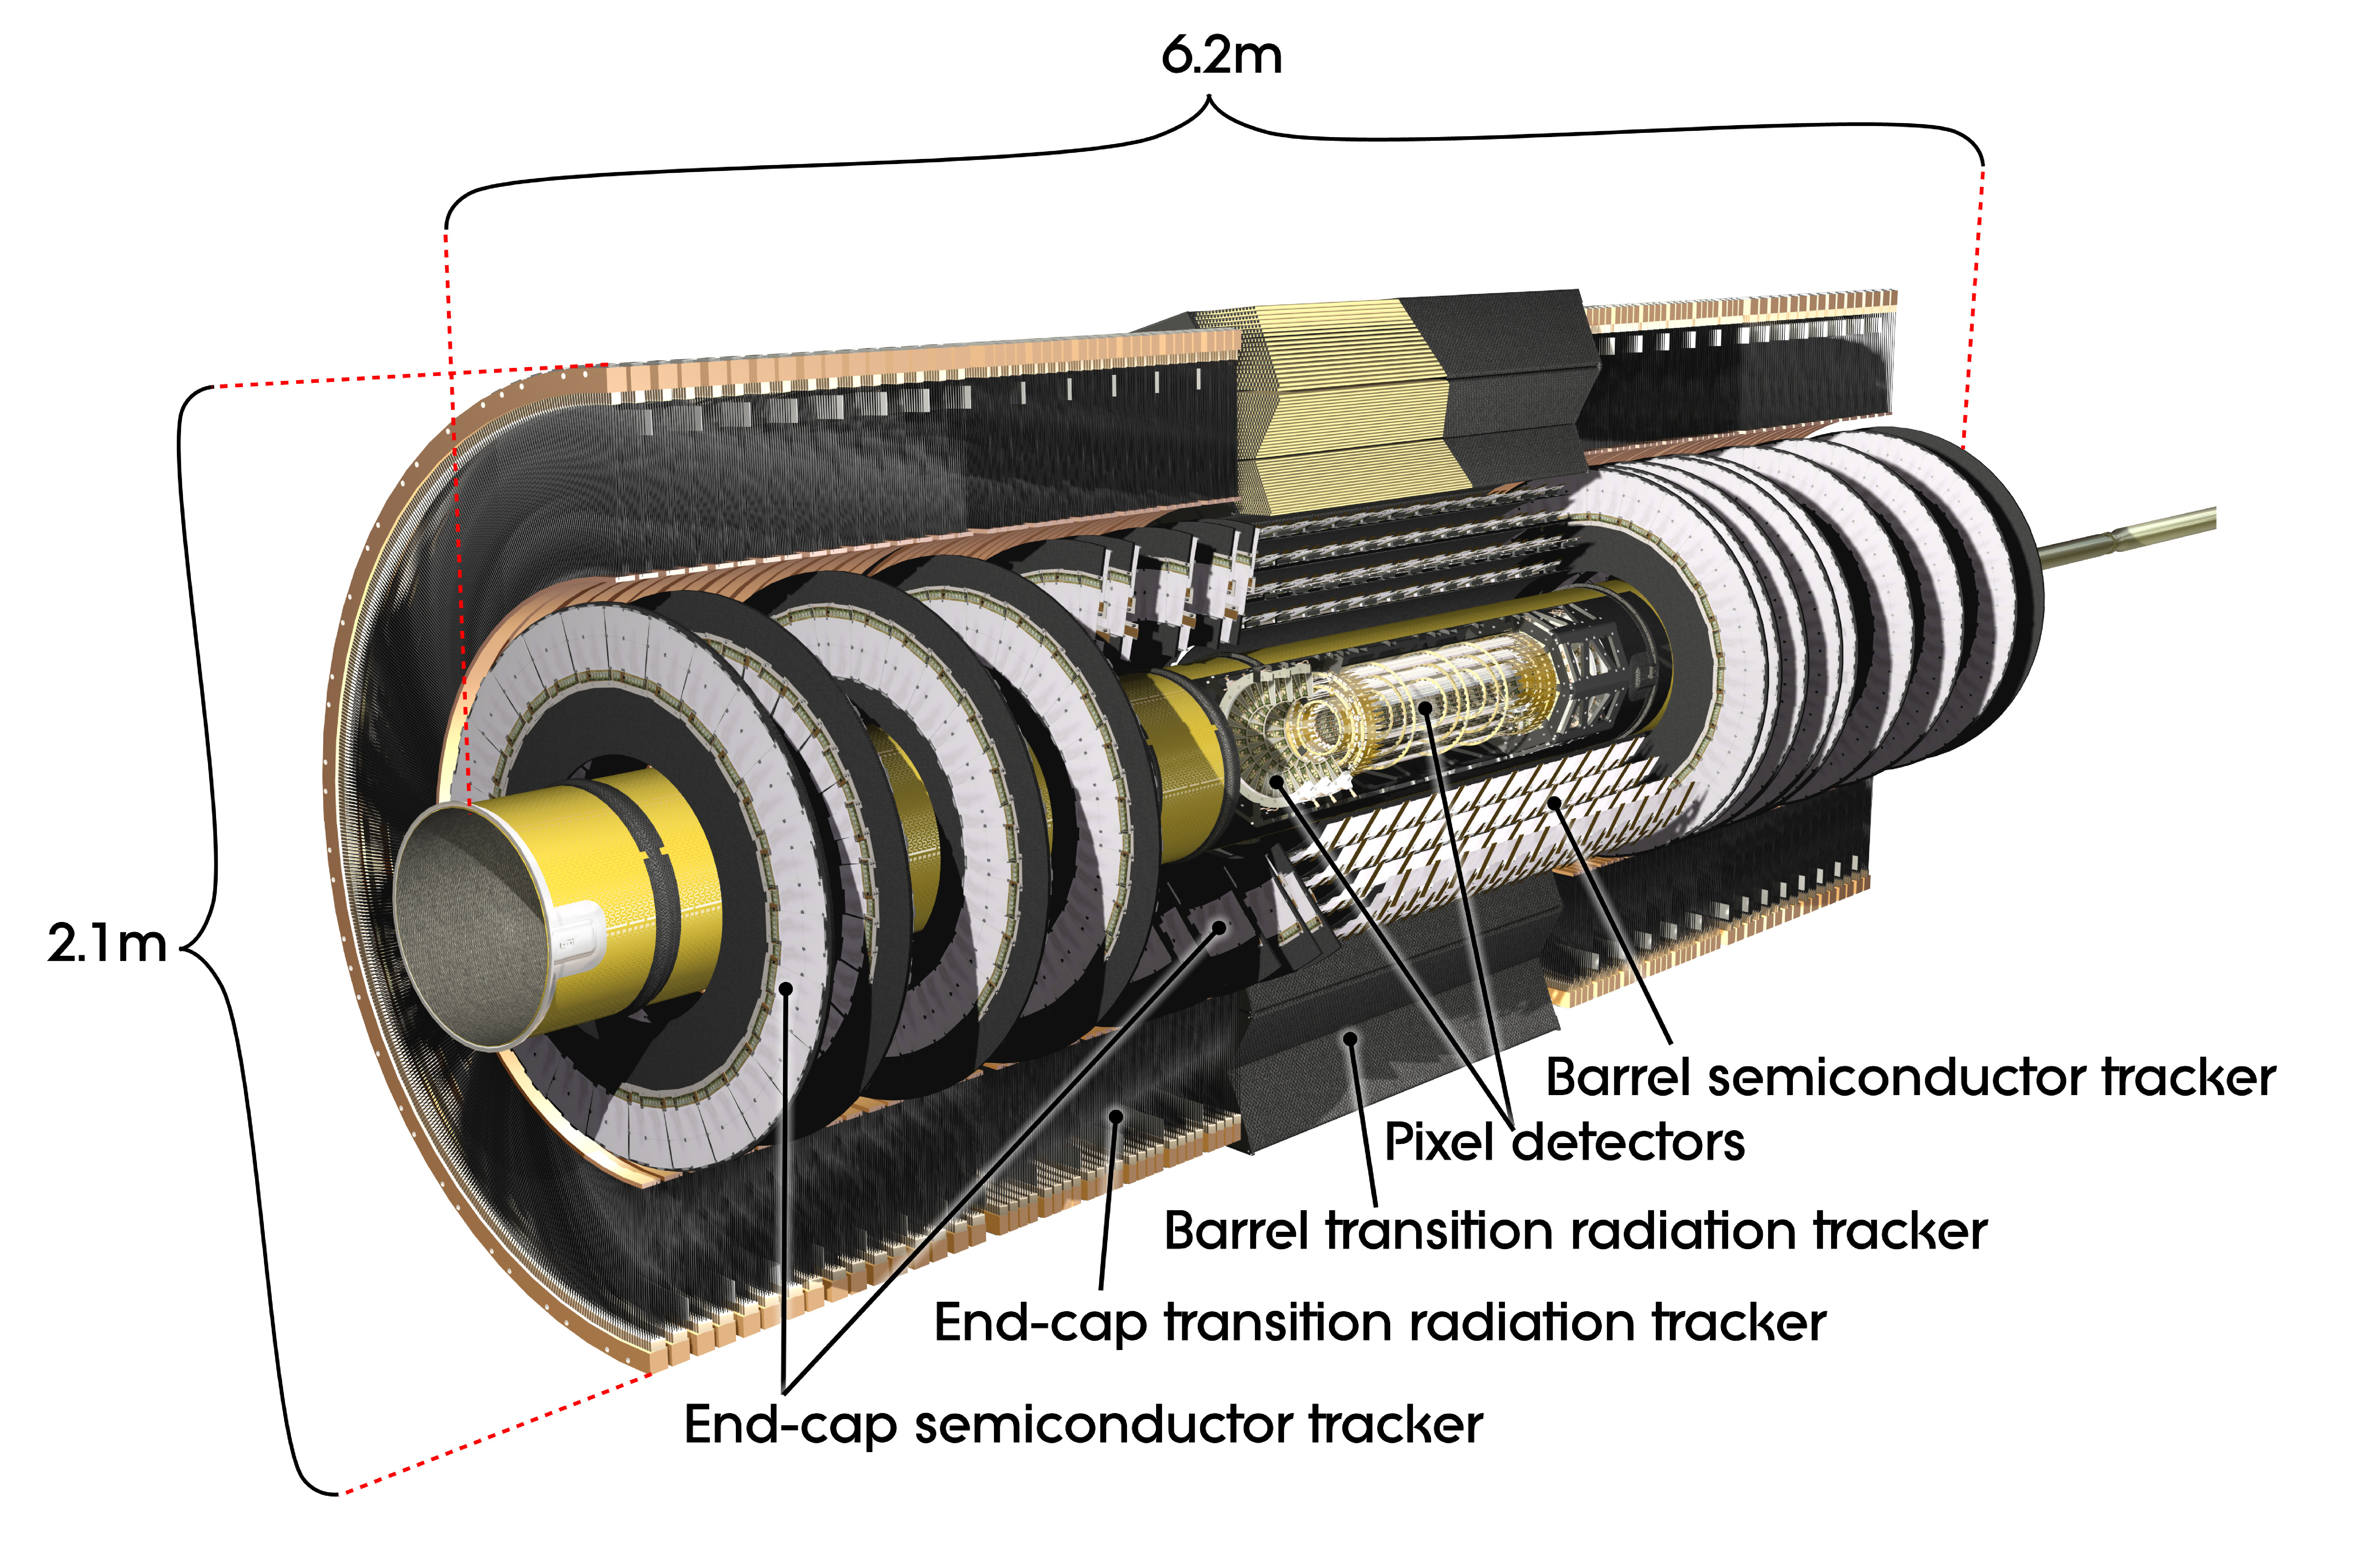
\includegraphics[width=0.70\textwidth]{ID-eps-converted-to.pdf}
\caption{Esquema general del detector interno de ATLAS.}
\label{ID}
\end{figure}

\tosolve{tamaño de pixel s resolucion}

El detector interno (Figura \ref{ID}) es el más próximo al haz y combina detectores de muy alta resolución con detectores continuos de trazas. Está contenido dentro del solenoide que provee un campo magnético de $2$ T. Los distintos detectores que lo componen se describen a continuación. Se puede ver un corte transversal de los mismos en la Figura \ref{ID_2}.

\begin{figure}
\centering
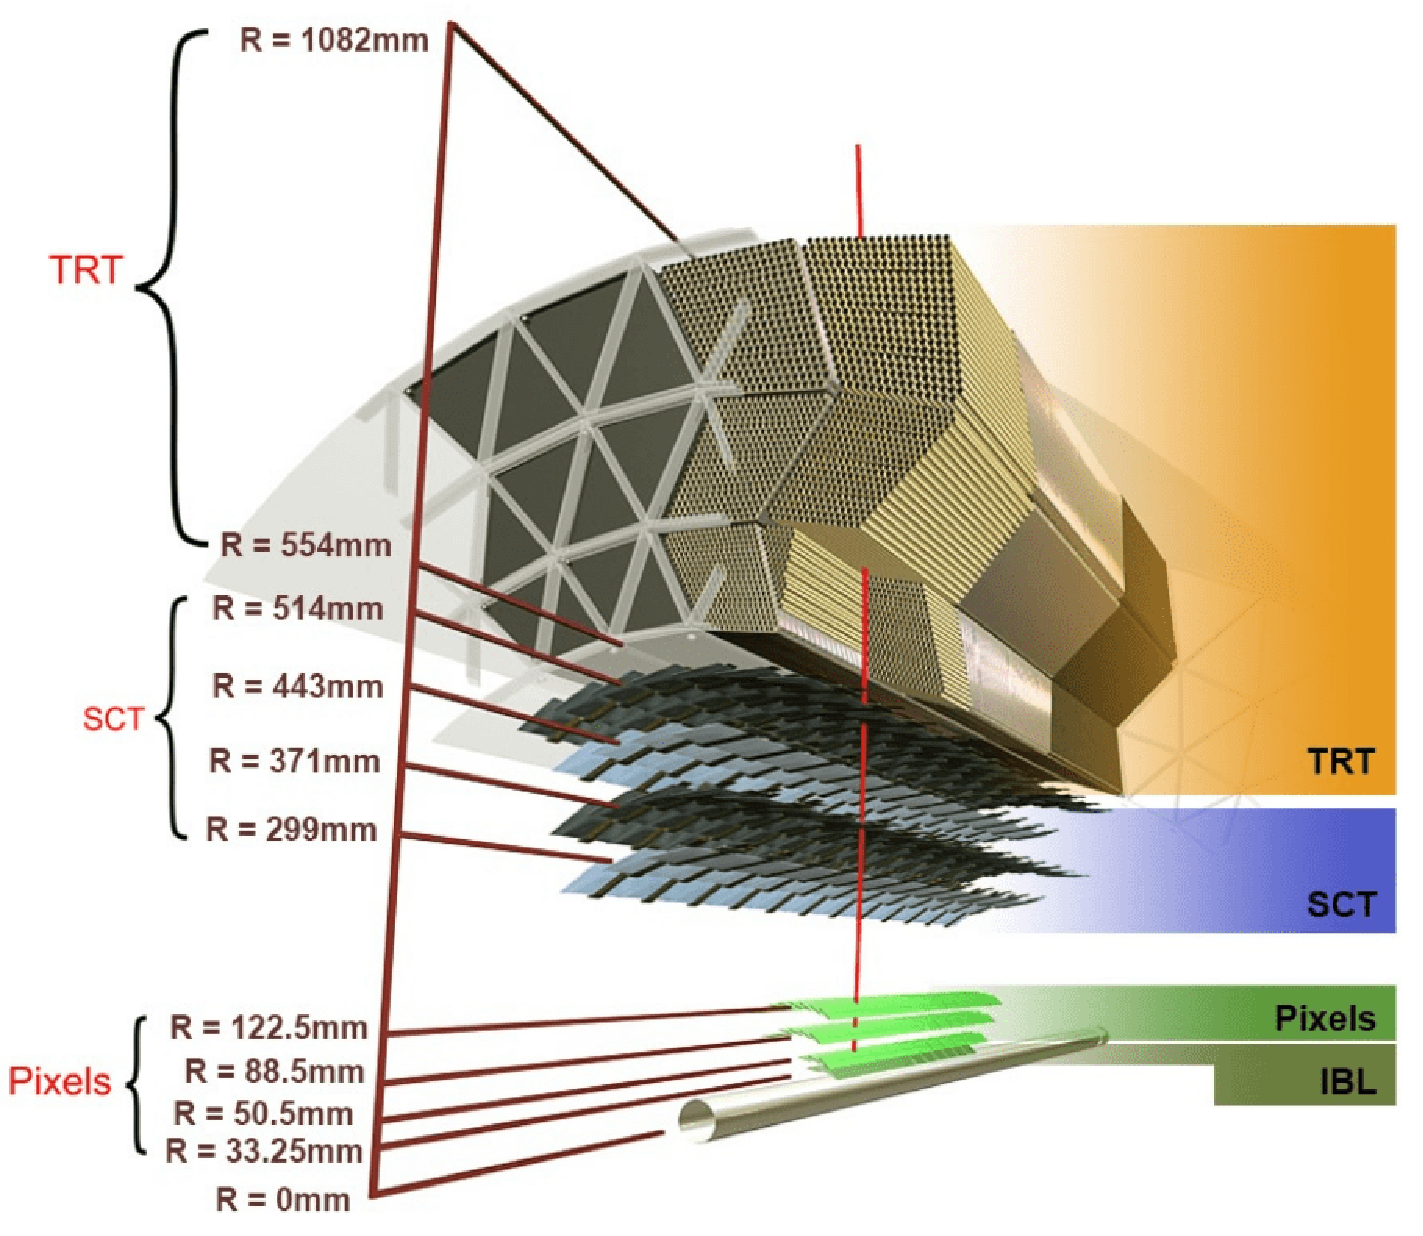
\includegraphics[width=0.60\textwidth]{ID_2.pdf}
\caption{Esquema del detector interno mostrando la traza de una partícula cargada de $p_{T}=10 \egev$ atravesándolo. La trayectoria atraviesa el tubo del haz de  berilio, las tres capas del detector de píxeles de silicio, las cuatro capas dobles del SCT, y aproximadamente 36 tubos contenidos en los módulos del TRT.}
\label{ID_2}
\end{figure}
% \vspace{0.5cm}

\subsubsection{Insertable B-Layer}

Luego del Run 1 la luminosidad del LHC aumentó notablemente, lo que podía significar un daño por radiación en los detectores internos. En vez de reemplazar las partes del detector de píxeles que podían ser dañadas, se decidió colocar una capa insertable entre el detector de píxeles y la tubería donde circulan los protones. El objetivo del mismo es mejorar la eficiencia en la identificación de trazas, vértices, y en la identificación de bottom quarks, que decaen típicamente fuera del radio del IBL.

El IBL está compuesto por $8$ millones de chips de rápida lectura y con sensores de silicio, que detectan el paso de partículas cargadas mediante la deposición de carga inducida. El tamaño de los píxeles es de $50\times250\:\mu$m$^{2}$, con una resolución de $8\:\mu$m ($R-\phi$) y $40\:\mu$m ($z$). La distancia entre el IBL y la tubería es de $0.2$ mm, y entre el tubo y el detector de píxeles es de $1.9$ mm. 

\subsubsection{Detector de píxeles}

El detector de píxeles fue construido para medir la posición de las trazas de partículas cargadas con la más alta precisión posible y es de vital importancia para la reconstrucción de los vértices primarios y secundarios. En la región \textit{barrel} el detector se compone de tres capas cilíndricas, mientras que la \textit{endcap} de tres discos. La capa más interna, denominada \textit{B-Layer}, se encuentra a $50.5$ mm del punto de interacción. El principio de detección para partículas cargadas es la medida de la deposición de la carga inducida en una capa de silicio por ionización. El sistema contiene un total de $80$ millones de sensores, cada uno con una resolución de $10\:\mu$m ($R-\phi$) y $115\:\mu$m ($z$).

\subsubsection{Detector Semiconductor de Trazas (SCT)}

Se encuentra por fuera del detector de píxeles y está diseñado para medir las trazas con alta precisión en la zona intermedia del detector. A diferencia del detector de píxeles, estos sensores de silicio están segmentados en micro bandas, dada la más baja multiplicidad de partículas. La resolución de $17\:\mu$m ($R-\phi$) y $580\:\mu$m ($z$). En la región \textit{barrel} los módulos de SCT están dispuestos en 4 capas concéntricas, mientras que en la región \textit{endcap} consiste en 9 discos transversales al eje del haz.

\subsubsection{Detector de Radiación de Transición (TRT)}

Es el detector más externo del ID y está diseñado, no solo para detectar partículas cargadas, sino también para distinguir entre partículas pesadas y livianas. El TRT se compone de tubos detectores de $4$ mm de diámetro, con un gas que ioniza al ser atravesado por partículas cargadas. Los electrones producidos son colectados por una ánodo, y el tiempo de deriva es una medida de la distancia a la traza del mismo.  Además, los tubos están rodeados de fibras de polipropileno con un índice de refracción diferente, por lo que las partículas que atraviesan el detector emiten radiación con una intensidad proporcional a $\gamma=E/m$. De esta forma, el TRT permite distinguir partículas cargadas pesadas ($\pi^{\pm}$) de aquellas más livianas ($e^{\pm}$). La región \textit{barrel} contiene $50000$ tubos paralelos al eje del haz y la región \textit{endcap} $320000$ tubos orientados radialmente. Su resolución es de $0.17$ mm.

\subsection{Calorímetros}

El sistema de calorímetros de ATLAS está diseñado para medir la energía y la posición de las partículas, mediante la absorción de la energía depositada por las cascadas de partículas secundarias que estas generan en el material del mismo. Además, permite discriminar electrones y fotones de jets, medir el desbalance de energía transversa y la selección online de eventos potencialmente interesantes (\textit{trigger}). Este sistema incluye un calorímetro electromagnético (ECAL) y otro hadrónico (HCAL), como muestra la Figura \ref{Cal}.

\begin{figure}
\centering
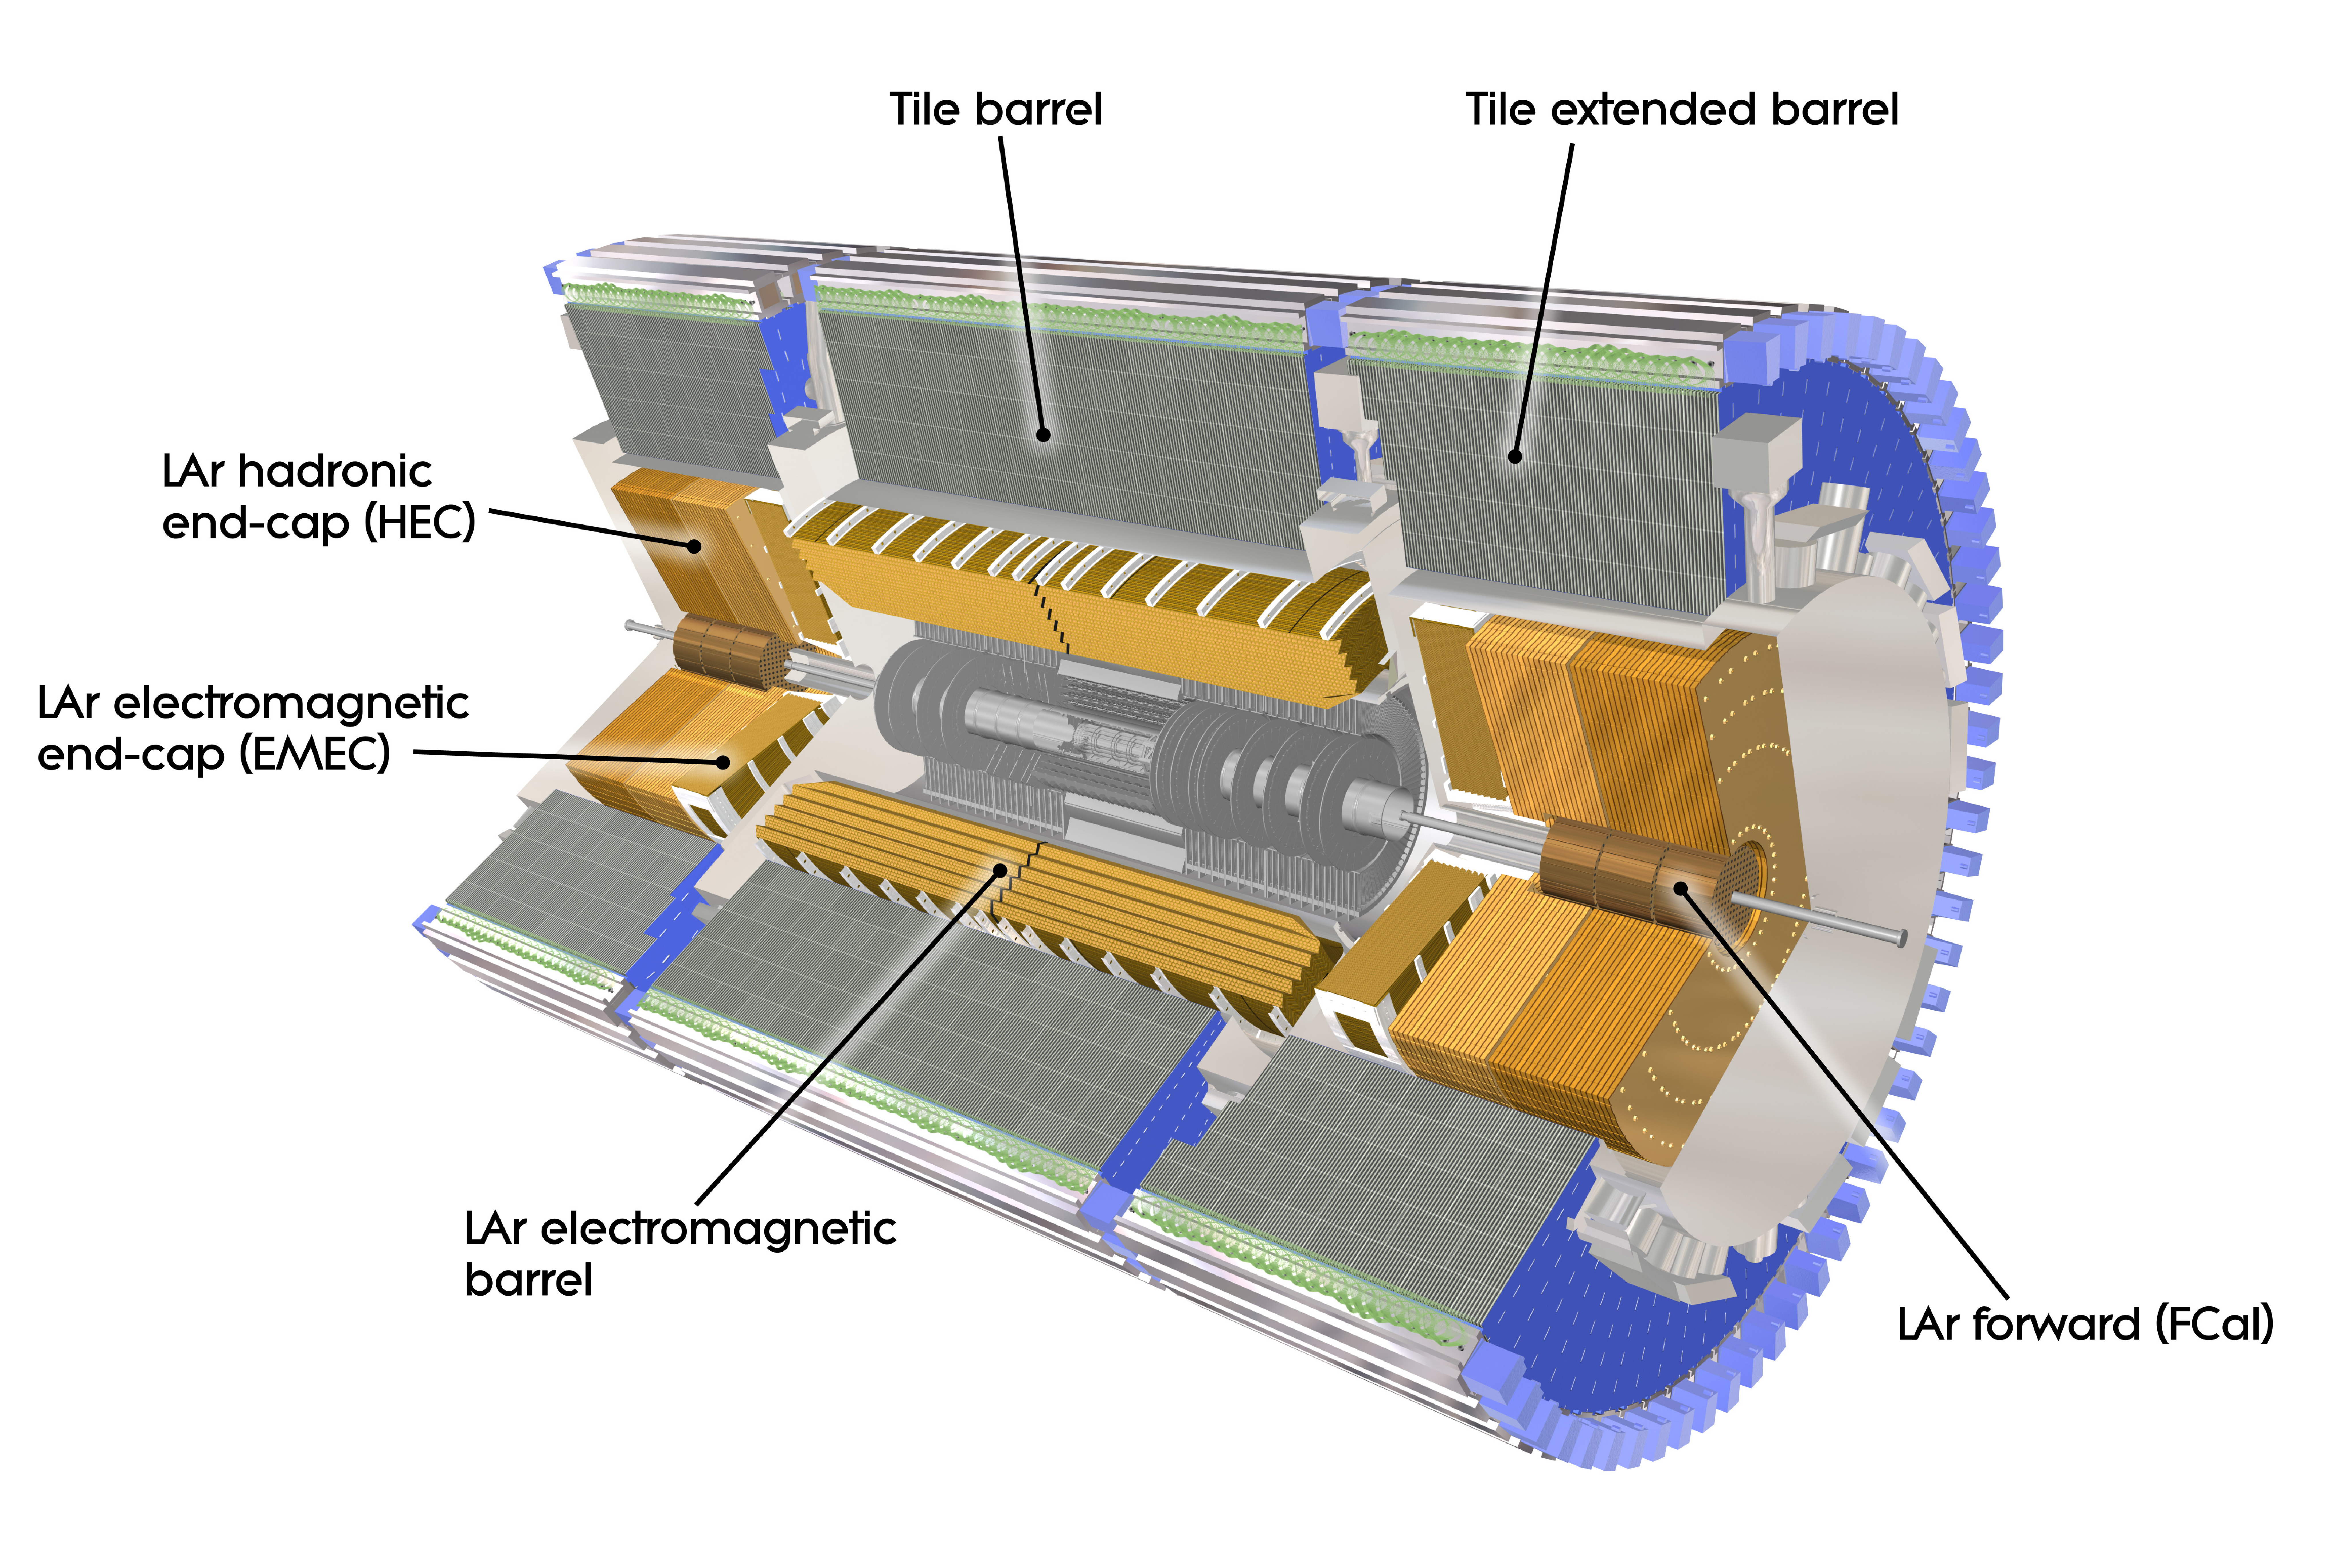
\includegraphics[width=0.70\textwidth]{Cal-eps-converted-to.pdf}
\caption{Sistema de calorímetros del detector ATLAS.}
\label{Cal}
\end{figure}

\subsubsection{Calorímetro electromagnético (ECAL)}

El ECAL en un calorímetros de muestreo inhomogéneo no compensado, que utiliza plomo como material absorbente. Las partículas incidentes interactúan con este material creando una lluvia de partículas cargadas y neutras. Las partículas cargadas ionizan el medio activo (LAr) colocado entre las placas de plomo, donde los electrones liberados son colectados en un electrodo central de kaptón/Cu hacia donde derivan por acción del campo eléctrico aplicado. La señal total en el medio activo es así proporcional a la energía total real de la partícula incidente.

% \begin{figure}
% \centering
% 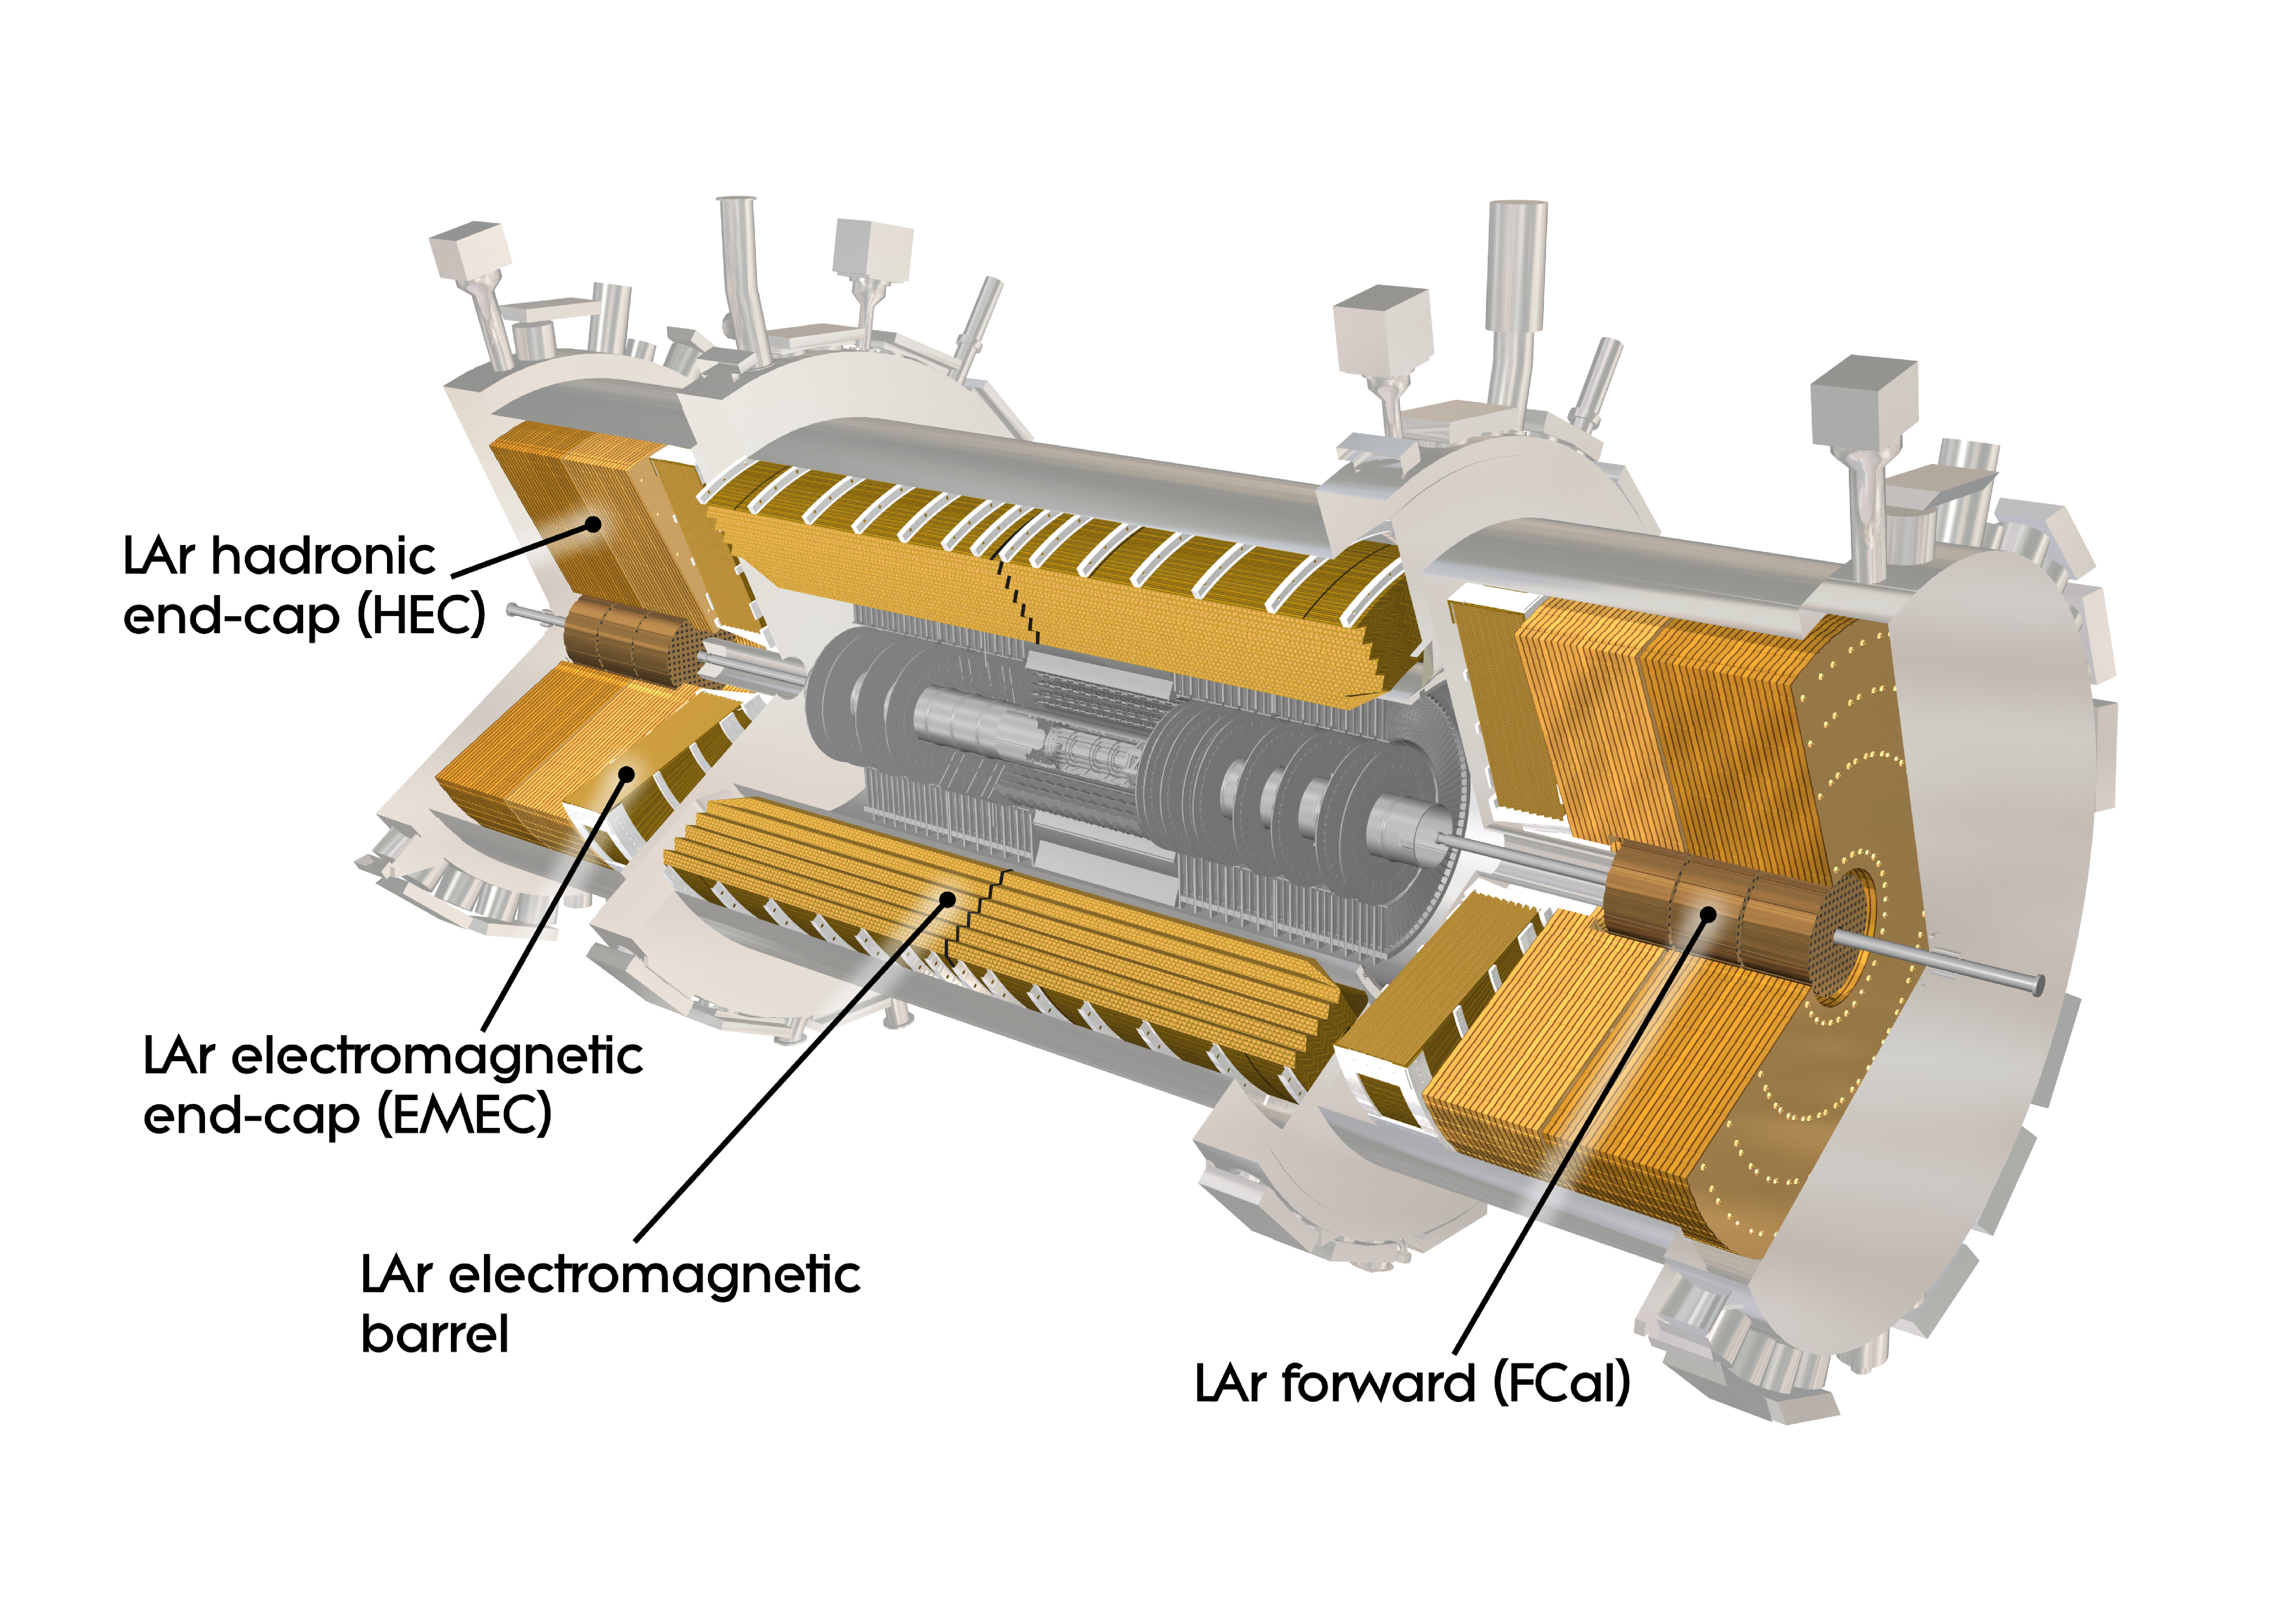
\includegraphics[width=0.70\textwidth]{ecal.eps}
% \caption{ECAL del detector ATLAS.}
% % \vspace{0.2cm}\footnotesize\textbf \sl{...}\vspace{0.2cm}
% \label{ecal}
% \end{figure}

El ECAL se divide en una parte central (\textit{barrel}) y dos \textit{endcaps} a cada lado. En la región de transición entre el \textit{barrel} y el \textit{endcap} se encuentra una zona no instrumentada, por donde se conecta el detector. Esta región, denominada \textit{crack}, está comprendida entre $1.37 < |\eta| < 1.52$. Es por este motivo que la mayoría de los análisis se requiere que los candidatos a fotones/electrones estén fuera de la región \textit{crack}.

\subsubsection{Calorímetro hadrónico (HCAL)}

El HCAL es un conjunto de calorímetros que rodean al ECAL. El primero de los calorímetros se denomina \textit{Tile Calorimeter}, es un calorímetro de muestreo que utiliza acero como material absorbente y tejas centelladoras plásticas como material activo. En la región \textit{endcap} se encuentra un calorímetro hadrónico de muestreo (HEC) con placas de cobre como absorbente y argón líquido como material activo, que consiste en dos ruedas, una atrás de la otra. Finalmente se encuentra el Forward Calorimeter (FCAL), un calorímetro de muestreo que extiende la cobertura del sistema a $|\eta|<4.9$. Estos detectores extienden la aceptancia del calorímetro de ATLAS hasta cubrir prácticamente la totalidad de ángulo sólido del punto de colisión.

% El calorímetro hadrónico cubre el rango $|\eta|< 4.9$ usando diferentes materiales. La parte del \textit{barrel} de este sistema utiliza acero como absorbente y tejas centelladoras como material activo. Las tejas están ubicadas radialmente y apiladas en profundidad. En la región de \textit{endcaps}, el calorímetro hadrónico se compone de dos ruedas perpendiculares al tubo del haz, hechas con placas de cobre y tungsteno como material absorbente y argón líquido como material activo. Estos detectores extienden la aceptancia del calorímetro de ATLAS hasta cubrir prácticamente la totalidad de ángulo sólido del punto de colisión.

\subsection{Espectrómetro de muones (MS)}

Los muones de alto $p_{T}$ generados en el punto de interacción tienen un altísimo poder de penetración y son poco interactuantes. Por ello el espectrómetro de muones se encuentra situado en la parte más exterior del detector ATLAS, siendo los muones las únicas partículas que llegan a él. Se encuentra alrededor del sistema de imanes de toroides, y está diseñado para obtener mediciones de alta precisión de la posición e impulso de los muones, y para una rápida identificación para el sistema de \textit{trigger}. Este es el subdetector más grande y el que le da a ATLAS su tamaño característico. 

El MS se compone de diferentes tipos de cámaras de detección de muones (ver Figura \ref{muon}). Las \textit{Monitored Drift Tubes} (MDTs) son responsables de la mayoría de las medidas de precisión. Funcionan de forma similar al TRT, con tubos llenos de un gas que ioniza y un ánodo central que recoge los electrones producidos, y el tiempo de deriva se asocia con la distancia a la traza. En la región \textit{endcap} se encuentran las \textit{Cathode Strip Chambers} (CSCs) que poseen alta resolución espacio-temporal. Estas cámaras funcionan midiendo la carga depositada en un ánodo, producto de la cascada de electrones creados cerca del mismo. Las \textit{Resistive Plate Chamber} (RPCs) proveen una estimación rápida del momento de los muones al primer nivel del \textit{trigger}. Las RPCs miden la descarga ocasionada entre dos placas resistivas paralelas sometidas a una alta diferencia de potencial, tras la ionización del volumen de gas interno causada por el paso de muones energéticos. Finalmente se encuentra las \textit{Thin Gap Chambers} (TGCs), similares en funcionamiento a las CSCs. Se encuentran en la región \textit{endcap} y proveen también información al sistema de \textit{trigger} en esta región.


\begin{figure}
\centering
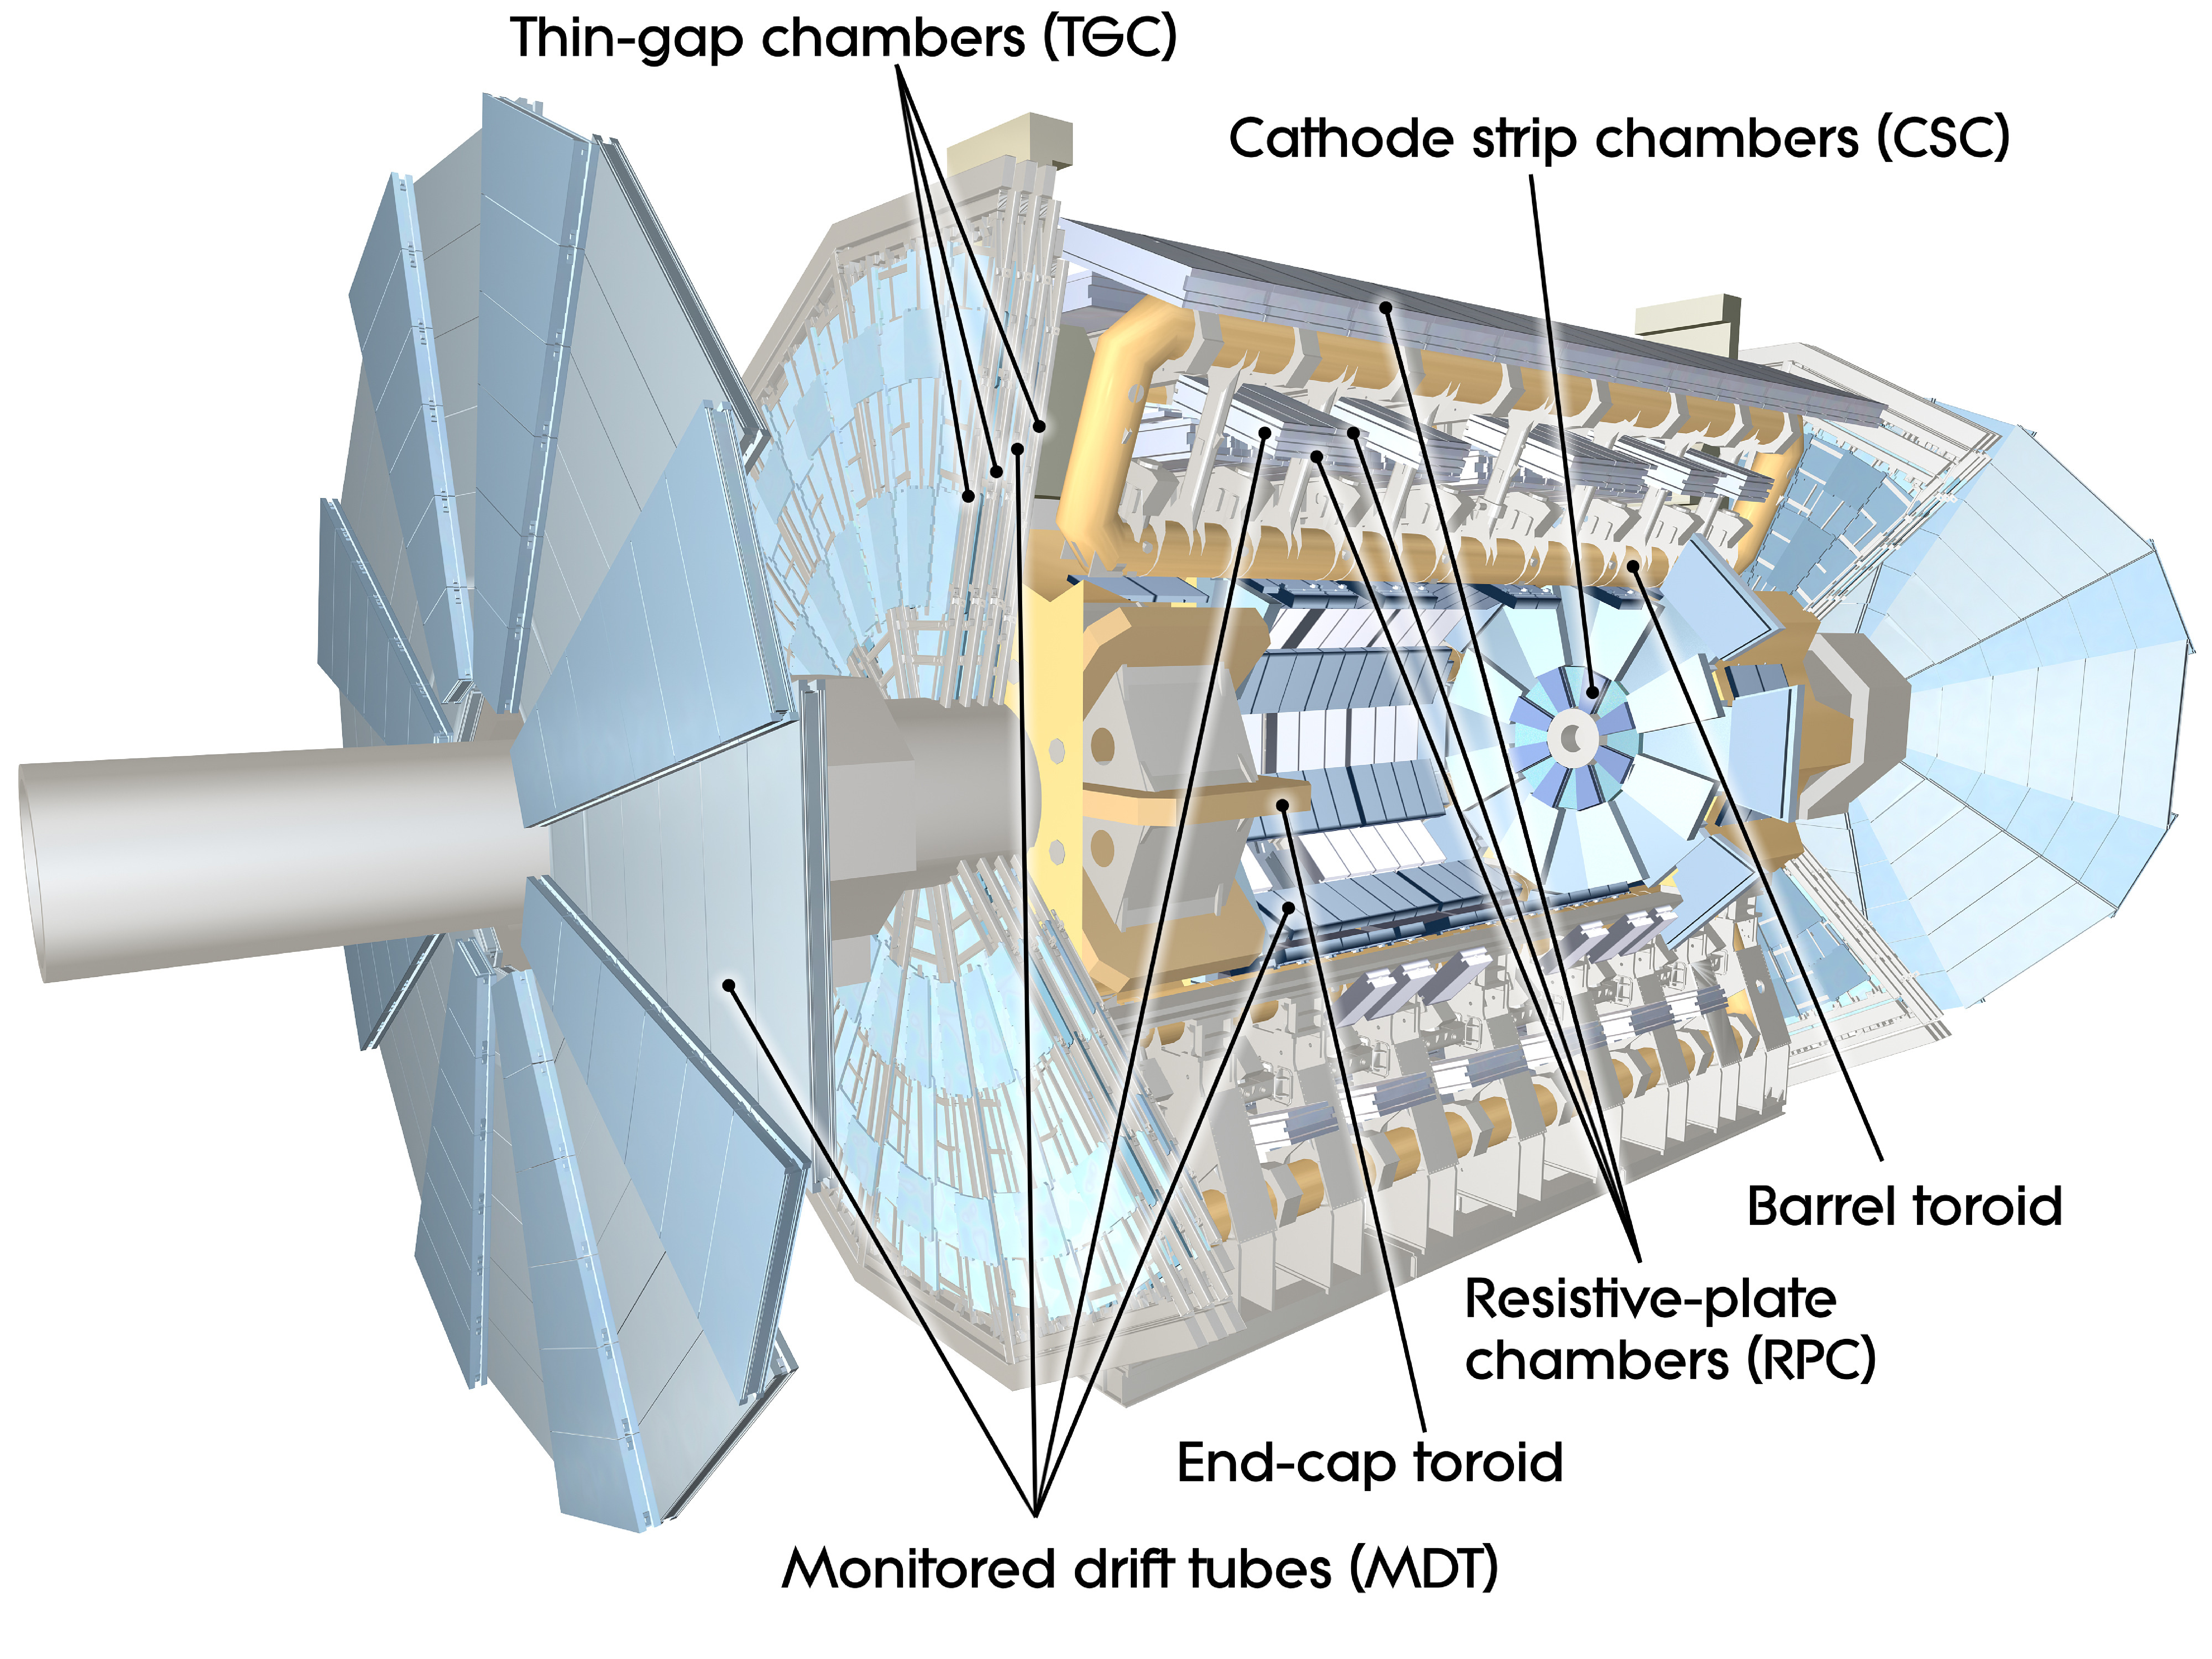
\includegraphics[width=0.60\textwidth]{muon-eps-converted-to.pdf}
\caption{Espectrómetro de muones del detector ATLAS.}
\label{muon}
\end{figure}



\section{Sistema de \textit{trigger}}

El diseño del LHC permite tener una frecuencia de cruces de haces de 40 MHz y alrededor de 23 interacciones por cruce, lo que da una tasa de interacción protón-protón del orden del GHz. Debido a que el almacenamiento y el poder de cómputo de los datos recolectados son limitados, y considerando que no todos los eventos son de interés, es necesario reducir el flujo de datos incidentes a una frecuencia de $\sim 1.5$ kHz \cite{PERF-2011-02}. El sistema de trigger, es el encargado de filtrar los eventos que son de interés, para su posterior análisis. 

El sistema de trigger de ATLAS consiste en una selección de eventos basada en dos niveles: Level 1 (L1) y el \textit{High Level Trigger} (HLT). Cada nivel permite analizar los eventos con mayor detalle, aumentando así la precisión de los criterios de selección y la complejidad de los algoritmos utilizados.



El primer nivel de trigger se encarga de la selección inicial, reduciendo la frecuencia de eventos que pasan al siguiente nivel a $\sim100$ kHz. Debido al tamaño limitado de las memorias temporales donde se guardan los datos de cada subdetector y al considerable tiempo de vuelo de las partículas hasta el espectrómetro de muones, la decisión debe tomarse en una escala de tiempo muy limitada ($2.5 \:\mu$s). El L1 está basado en hardware y selecciona objetos de alto $p_{T}$ construidos a partir de la información de varios subdetectores. Ciertas celdas del ECAL y el HCAL se utilizan entonces para enviar señales al L1 con información de los objetos. La posición de cada objeto encontrado define una <<región de interés>> (RoI) en un evento potencialmente interesante, que se extiende como un
cono desde el punto de interacción a lo largo del detector. Lo mismo en el detector de muones, que tiene diferentes cámaras que permiten obtener una estimación rápida del $p_{T}$ de los muones. El diseño del L1 le permite tener una aceptancia en el rango de $|\eta|<2.5$ para electrones, fotones, muones y taus; hasta $|\eta|<3.2$ para jets y $|\eta|<4.9$ para el cálculo de la energía transversa perdida.


Si el evento es aceptado por el L1 todos los datos y las ROIs pasan al \textit{High Level Trigger}. El HLT realiza la decisión final utilizando algoritmos más complejos, teniendo acceso a toda la información del evento en los distintos subdetectores de ATLAS, con la máxima granularidad e incluyendo detalles sobre la calibración de energía de los calorímetros, la alineación de los subdetectores y el mapa de campo magnético. De esta forma se reduce la frecuencia de eventos hasta  $\sim 1.5$ kHz en un tiempo de $0.2$ s. El tiempo de latencia disponible para tomar la decisión final sobre el evento permite la reconstrucción completa del mismo, y el refinamiento de las variables y criterios de selección al nivel de aquellos implementados en el análisis \textit{offline}. Los eventos aceptados por el HLT son finalmente grabados a disco y distribuidos, accesibles \textit{offline} para todos los análisis subsecuentes.

% El segundo nivel del trigger (L2) se centra únicamente en las RoIs donde el L1 encontró actividad, combinando información de todos los subdetectores dentro de cada una ($\sim2$ \% de la cobertura total del detector). El L2 consiste de una serie de algoritmos de reconstrucción y selección especializados, diseñados para reducir la frecuencia de eventos hasta aproximadamente 1 kHz. Estos algoritmos están implementados en \textit{clusters} de procesamiento dedicados que analizan cada evento dentro de un tiempo de latencia medio de $\sim40$ ms. El menor flujo de información en este nivel del trigger permite calcular las variables calorimétricas con mayor precisión y hacer uso de la información de las trazas reconstruidas, haciendo posible la distinción entre fotones y electrones, y el rechazo de fondo proveniente en su mayoría de jets.
% La última etapa de la selección del trigger se lleva a cabo en el \textit{Event Filter}, que reduce la frecuencia de eventos a $\sim 1.5$ kHz. En este nivel se tiene acceso a toda la información del evento en los distintos subdetectores de ATLAS, con la máxima granularidad e incluyendo detalles sobre la calibración de energía de los calorímetros, la alineación de los subdetectores y el mapa de campo magnético. El tiempo de latencia relativamente largo disponible para tomar la decisión final sobre el evento ($\sim4$ s) permite la reconstrucción completa del mismo, y el refinamiento de las variables y criterios de selección al nivel de aquellos implementados en el análisis \textit{offline}. Los eventos aceptados por el EF son finalmente grabados a disco y distribuidos, accesibles \textit{offline} para todos los análisis subsecuentes.

Para cada ítem del trigger se puede asignar además un factor de escala o prescale (PS), que define la frecuencia con la que un dado ítem es evaluado por el trigger (es decir solo en uno de cada PS eventos). Se habla de una cadena de \textit{trigger unprescaled} si su factor de escala es PS = 1 en cada nivel, es decir, es evaluada en todos los eventos. La asignación de estos factores se hace incluso dinámicamente durante una toma de datos, para tener en cuenta el descenso de la luminosidad instantánea con el tiempo y mantener la tasa de procesamiento aproximadamente constante.

\section{Modelo computacional y distribución de datos}

La arquitectura computacional de ATLAS está diseñada para permitir a todos los miembros de la colaboración un acceso ágil, directo y distribuido a la gran cantidad de datos colectados por el detector ($\sim$ PB/año). La arquitectura se basa en la tecnología GRID \tosolve{cita}, compartiendo el poder de procesamiento y la capacidad de almacenamiento disponibles en distintos centros de cómputo asociados alrededor del mundo.

El software de ATLAS se desarrolla dentro un entorno C++ común llamado ATHENA \cite{ATLASComputing, Lenzi:1214931, Calafiura:865624}, en el que se realiza todo el procesamiento de datos. Los eventos aceptados por el trigger deben ser procesados para reducir su tamaño y ser utilizados para los análisis \textit{offline}. A la salida del HLT, los eventos son almacenados como \textit{Raw Data Objects} (RDOs). Luego de aplicar los algoritmos de reconstrucción y calibración, las colecciones de los distintos objetos físicos obtenidas son almacenadas en formato ESD (\textit{Event Summary Data}) y AOD (\textit{Analysis Object Data}), una versión reducida del primero ($\sim$100 kB/evento). A partir de las ESDs/AODs, se ha definido un formato de datos significativamente más pequeño (10-15 kB/evento) conocido como xAOD, sobre el que se realiza el análisis final. Las xAOD son archivos (<<ntuples>>), accesibles vía el entorno de análisis de datos ROOT \cite{Brun:1997pa}, que contienen un conjunto de variables para diferentes objetos físicos, según las necesidades de cada grupo de análisis dentro de ATLAS. 

Para agilizar el análisis final, la colaboración preselecciona eventos \textit{offline} en las llamadas derivaciones. Una de ellas, denominada EGAM1, utilizada en el presente trabajo, realiza una preselección de eventos optimizados para estudios del bosón $Z$, con una base de electrones y fotones con $p_{T} > 7 \egev$ y masa invariante de los distintos tipos de pares mayor a $50 \egev$, además de otras selecciones.